\documentclass[10pt,twocolumn,letterpaper]{article}

\usepackage[margin=0.75in]{geometry}
\usepackage[T1]{fontenc}
\usepackage[utf8]{inputenc}
\usepackage{times}
\usepackage{microtype}
\usepackage{graphicx}
\usepackage{amsmath,amssymb,amsfonts,bm}
\usepackage{booktabs}
\usepackage{multirow}
\usepackage{enumitem}
\usepackage{listings}
\usepackage[numbers,sort&compress]{natbib}
\usepackage[hidelinks]{hyperref}
\usepackage[nameinlink,capitalize]{cleveref}
\usepackage{mathtools}

\lstset{basicstyle=\ttfamily\scriptsize,breaklines=true,columns=fullflexible,keepspaces=true}

\title{HiVA: Hierarchical Variable-Horizon Actions for Long-Horizon VLA Control}
\author{Jongwoo Park}
\date{}

\begin{document}
\maketitle

\begin{abstract}
Action chunking improves consistency and amortizes expensive action generation in Vision-Language-Action (VLA) models, but most VLAs still execute a fixed number of micro-actions per model call, creating a brittle trade-off between responsiveness and smooth long-horizon execution. We propose HiVA, a hierarchical variable-horizon action representation for denoising-based VLAs, where each macro action is encoded by a predicted duration and compact B-spline trajectory coefficients that reconstruct smooth, variable-length micro-action sequences. The key idea is to make \emph{how many} micro-actions to execute and \emph{how} those actions are represented part of the same denoising action expert, rather than treating chunk length as a fixed hyperparameter. To make HiVA easy to integrate into existing denoising VLAs, we keep the pretrained multimodal conditioning path and the main denoising transformer block, and modify only lightweight action-side projection layers and output heads. The method is trained on dynamically relabeled macro-actions generated by a dynamic-programming oracle that favors segments that are both well approximated by B-splines and aligned with sub-task difficulty. We plan to evaluate the resulting representation on LIBERO-Plus and CALVIN by instantiating it in SmolVLA and VPP, covering different model scales (0.45B, 1.5B) and families (VLM, Diffusion backbones). The intended outcome is a smooth, compact, variable-horizon action representation that transfers across denoising VLA backbones and improves long-horizon manipulation.
\end{abstract}

\section{Related Work}

\paragraph{Action chunking and adaptive execution horizons.}
Action chunking has become a standard design choice in modern robot policies and VLAs because it improves temporal consistency and amortizes expensive action generation over multiple control steps \cite{act2023,diffusionpolicy2023,smolvla2025,vpp2024}. However, fixed-horizon chunking exposes a persistent trade-off: longer executed chunks improve smoothness and reduce model calls, while shorter chunks improve responsiveness to new observations. Recent inference-time methods address this issue by changing how many actions from a predicted chunk are executed. AAC adapts chunk size using action entropy estimated from multiple sampled chunks, while AutoHorizon adjusts the executed prefix of a denoising-based VLA according to model confidence or attention-derived cues \cite{aac2026,autohorizon2026}. Real-time chunking and asynchronous execution methods further reduce pauses and boundary artifacts by generating future chunks while the current chunk is being executed \cite{rtc2025,abpolicy2026}. HiVA is complementary to these inference-time strategies, but differs in that the execution duration is learned as part of the action representation itself. Instead of selecting a prefix from a fixed raw-action chunk after prediction, HiVA predicts a duration-conditioned compact macro action in one denoising pass and decodes it into a variable-length sequence of native micro-actions.

\paragraph{Hierarchical RL and chunked action spaces.}
The idea of using temporally extended actions is closely related to hierarchical reinforcement learning, where high-level decisions select options, skills, subgoals, or other abstractions that persist for multiple environment steps \cite{options1999,hiro2018,hac2019}. These methods improve long-horizon decision making by reducing the effective planning horizon and allowing the policy to reason over behavioral segments rather than individual low-level controls. More recent work on action chunking for RL shows that directly operating in a temporally extended action-sequence space can improve exploration and temporal-difference learning in long-horizon sparse-reward settings \cite{qchunking2025}. HiVA shares this temporal-abstraction perspective, but targets denoising-based VLA action experts rather than RL critics or separately learned option policies. In HiVA, a macro action is not a symbolic skill or independent high-level policy output; it is a duration-conditioned compact code predicted by the same action expert and decoded into native robot micro-actions.

\paragraph{Smooth and compact action representations.}
Another line of work studies action representations that are smoother or more compact than raw per-step action sequences. Diffusion policies and action-chunking transformers model multi-step action sequences directly, but they often operate in the raw action space and therefore inherit issues such as intra-chunk jitter, inter-chunk discontinuity, or sensitivity to the chosen horizon \cite{act2023,diffusionpolicy2023,aac2026,abpolicy2026}. Function-space representations address this issue by parameterizing trajectories with compact bases. BEAST encodes action sequences into B-spline tokens, showing that B-spline representations can compress action chunks and generate smooth high-frequency control signals efficiently \cite{beast2025}. ABPolicy predicts continuous B-spline control points with a flow-matching policy and uses asynchronous refitting to improve real-time smoothness and inter-chunk continuity \cite{abpolicy2026}. 

HiVA builds on this evidence but uses B-splines differently. We relabel the training dataset into macro-actions and train the model to learn the duration within which a B-spline code can accurately approximate the underlying micro-action sequence. Thus, the duration is not merely an inference-time heuristic; it is a supervised prediction target coupled to the compact trajectory code. We also avoid forcing all action dimensions into a single homogeneous representation. Translation and rotation are treated as separate smooth cumulative trajectories with B-spline coefficient heads, while the gripper is represented as B-spline coefficients over the native continuous absolute command. This keeps the first coding path homogeneous across action modalities, while a sparse event-based gripper head remains a secondary ablation.

\paragraph{Denoising-based VLA action experts.}
Recent VLAs increasingly use dedicated action experts that condition diffusion or flow-matching policies on multimodal visual-language features \cite{smolvla2025,vpp2024,aac2026}. SmolVLA is a compact 0.45B VLA with a flow-matching action expert designed for efficient robotics, while VPP is a larger 1.5B-scale policy that conditions a diffusion policy on predictive visual representations from video modeling \cite{smolvla2025,vpp2024}. HiVA is designed for this modular setting. Rather than replacing the pretrained multimodal conditioner or the main denoising transformer block, it changes the action-side interface: fixed raw-action tokens and heads are replaced with duration, translation-coefficient, rotation-coefficient, and gripper heads. This makes HiVA a hierarchical variable-horizon action representation that can be tested across different denoising VLA backbones and model scales.


% \section{Motivation}
% Action chunking has become a standard design choice in modern VLAs because it improves temporal consistency and reduces the cost of replanning, but it also exposes a persistent trade-off: long executed chunks improve smoothness and reduce model calls, while short chunks improve responsiveness to new observations. AAC explicitly formulates this trade-off and argues that fixed chunk lengths hinder robustness across tasks; it adapts chunk size at inference time with action entropy estimated from multiple sampled chunks \cite{aac2026}. AutoHorizon reaches a closely related conclusion from a different angle: in denoising-based VLAs, performance can improve and then degrade as the executed prefix grows, so the execution horizon should be adjusted online rather than fixed once and for all \cite{autohorizon2026}. These observations motivate the central question of this paper: if chunk duration matters so much, should it remain an inference-time heuristic, or should it become a first-class prediction target of the action expert itself?

% Our answer is to learn the macro duration jointly with the chunk representation. Unlike AAC, which estimates duration indirectly from repeated test-time sampling, our approach predicts duration in one forward denoising pass and therefore avoids an extra inference-time chunk-search procedure \cite{aac2026}. Unlike AutoHorizon, which adjusts the executed prefix of an already predicted raw chunk using attention-based cues, our method changes the action representation itself: the action expert predicts a low-dimensional macro action that already encodes both the temporal extent and the shape of the chunk \cite{autohorizon2026}. In this sense, the method is complementary to test-time horizon adaptation, but more direct as a training objective.

% A second source of motivation is the emerging evidence that smooth function-space action representations are valuable. ABPolicy shows that predicting B-spline control points improves intra-chunk smoothness, but its design is centered on asynchronous action generation, continuity-constrained refitting, and online stitching between old and newly predicted chunks \cite{abpolicy2026}. BEAST similarly shows that B-spline tokenization can compress action sequences and generate smooth control signals efficiently \cite{beast2025}. Our setting is different. We are not trying to fit a B-spline over arbitrary windows or to continuously stitch asynchronously updated plans. Instead, we predict a macro duration precisely where a B-spline can represent the underlying micro-actions well, and we reconstruct those micro-actions in open loop within a single VLA call. This changes the role of the spline: it is not merely a smoother post hoc trajectory fit, but the native action representation used by the expert.

% This view leads to three design principles. First, duration prediction should be learned explicitly rather than searched at test time. Second, the action representation should be hierarchical: a macro token should specify the chunk duration and a compact trajectory code, from which the micro-actions are reconstructed. Third, translation, rotation, and gripper behavior should not be forced into one homogeneous head, because they have different geometry and different temporal structure. Translation and rotation are naturally represented by smooth cumulative trajectories, while the gripper is better modeled as a sparse event process.

% To make the proposal practical, we target modular denoising-based VLAs whose action expert already has a separated multimodal conditioning path and a transformer-based denoising block. SmolVLA is a compact 0.45B VLA with a flow-matching action expert designed for efficient robotics \cite{smolvla2025}. VPP is a larger 1.5B-scale policy that conditions a diffusion policy on predictive visual representations derived from video modeling \cite{vpp2024}. Across these models, the common opportunity is the same: preserve the pretrained multimodal conditioner and the main denoising transformer block, and replace only a small set of action-side layers with duration, coefficient, and gripper heads. This is the sense in which the proposed method aims to be both a new action representation and an easily attachable action expert that generalizes across model-size scales.

\section{Method}
\subsection{Overview}
We replace direct micro-action generation with a macro-to-micro action expert. In general, a micro-action can be any robot-dependent native action vector $a_t\in\mathcal{A}\subset\mathbb{R}^{m}$, and a macro action is a duration-conditioned compact code $M_j=(d_j,z_j)$ that is decoded into an approximate variable-length sequence of native micro-actions $\hat a_{j,1:d_j}=\mathcal{D}_{d_j}(z_j)$. In this paper, we instantiate this framework for 7-DoF end-effector control, where $z_j$ is represented by B-spline trajectory coefficients for translation, rotation, and the continuous gripper command. Specifically, for macro token $j$, the expert predicts
\begin{equation}
M_j = \bigl(d_j,\,\Theta^{\mathrm{tr}}_j,\,\Theta^{\mathrm{rot}}_j,\,\Theta^{\mathrm{grip}}_j\bigr),
\end{equation}
where $d_j\in\{1,\dots,D_{\max}\}$ is a discrete duration, $\Theta^{\mathrm{tr}}_j$ are B-spline coefficients for chunk-relative cumulative translation, $\Theta^{\mathrm{rot}}_j$ are B-spline coefficients for chunk-relative cumulative rotation, and $\Theta^{\mathrm{grip}}_j$ are B-spline coefficients for the absolute gripper command. Micro-actions are reconstructed from these macro parameters rather than generated independently. Because the macro action is a lower-dimensional representation of the original micro-action sequence, the B-spline reconstruction is not expected to be exactly identical to the expert trajectory. Instead, it provides a compact approximation whose reconstruction error is explicitly modeled during training. Our dynamic-programming relabeling therefore favors segments that can be represented accurately by the B-spline code while still allowing a controlled approximation loss.

\begin{figure*}[t]
    \centering
    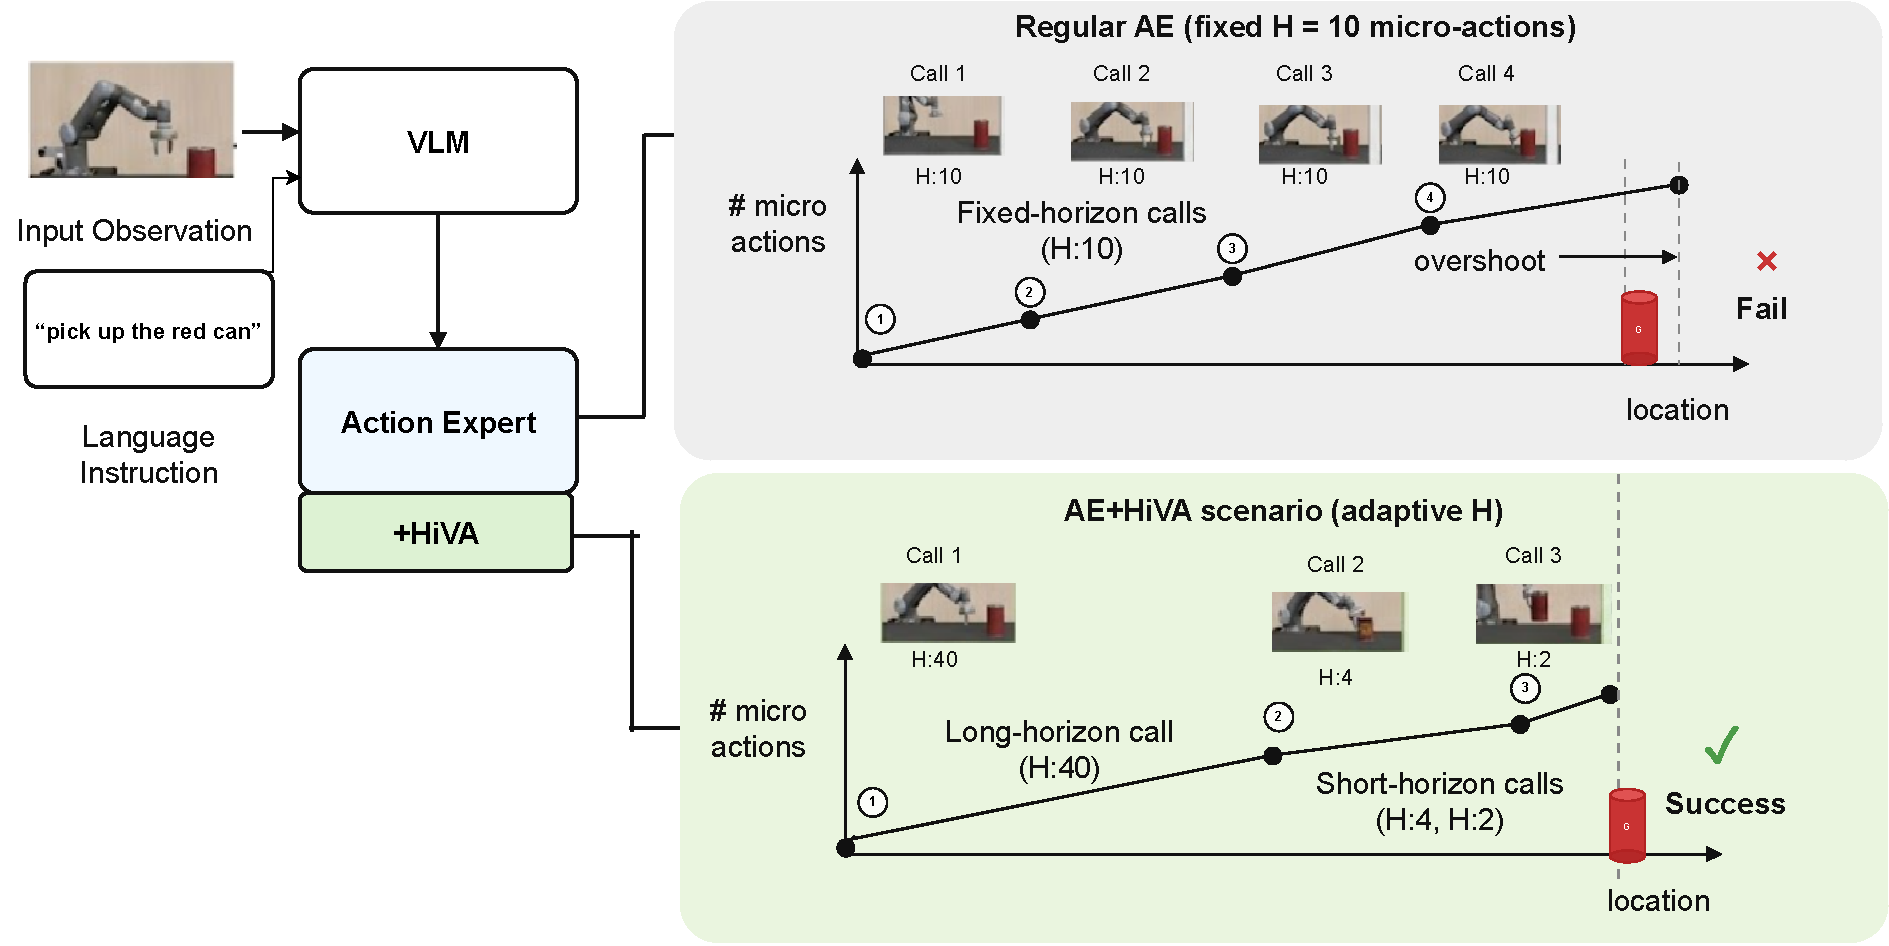
\includegraphics[width=0.98\textwidth]{HiVA_overview.pdf}
    \caption{Overview of HiVA. A regular action expert (AE) executes a fixed number of micro-actions for every model call. This fixed-horizon design can waste calls during easy free-space motion and still remain insufficiently reactive near the target object, causing overshoot and task failure. AE+HiVA instead predicts variable-horizon macro actions: longer horizons for easy sub-trajectories and shorter horizons for difficult, contact-sensitive manipulation. This lets the policy spend fewer calls on simple motion while increasing reactivity near the object, leading to successful long-horizon execution.}
    \label{fig:hiva-overview}
\end{figure*}

\Cref{fig:hiva-overview} illustrates the motivation behind the macro-to-micro design. With a fixed-horizon action expert, every call commits to the same number of micro-actions regardless of local task difficulty. In easy free-space motion, this wastes model calls because the robot could safely move farther before replanning. Near the target object, however, the same fixed horizon can be too coarse: the policy may continue executing an outdated chunk, overshoot the desired grasp region, and fail the task. HiVA addresses this by making the action horizon part of the predicted macro action. The action expert can therefore output a long macro-action for simple approach motion and shorter macro-actions for delicate manipulation, balancing inference efficiency with local reactivity.

\begin{figure}[t]
    \centering
    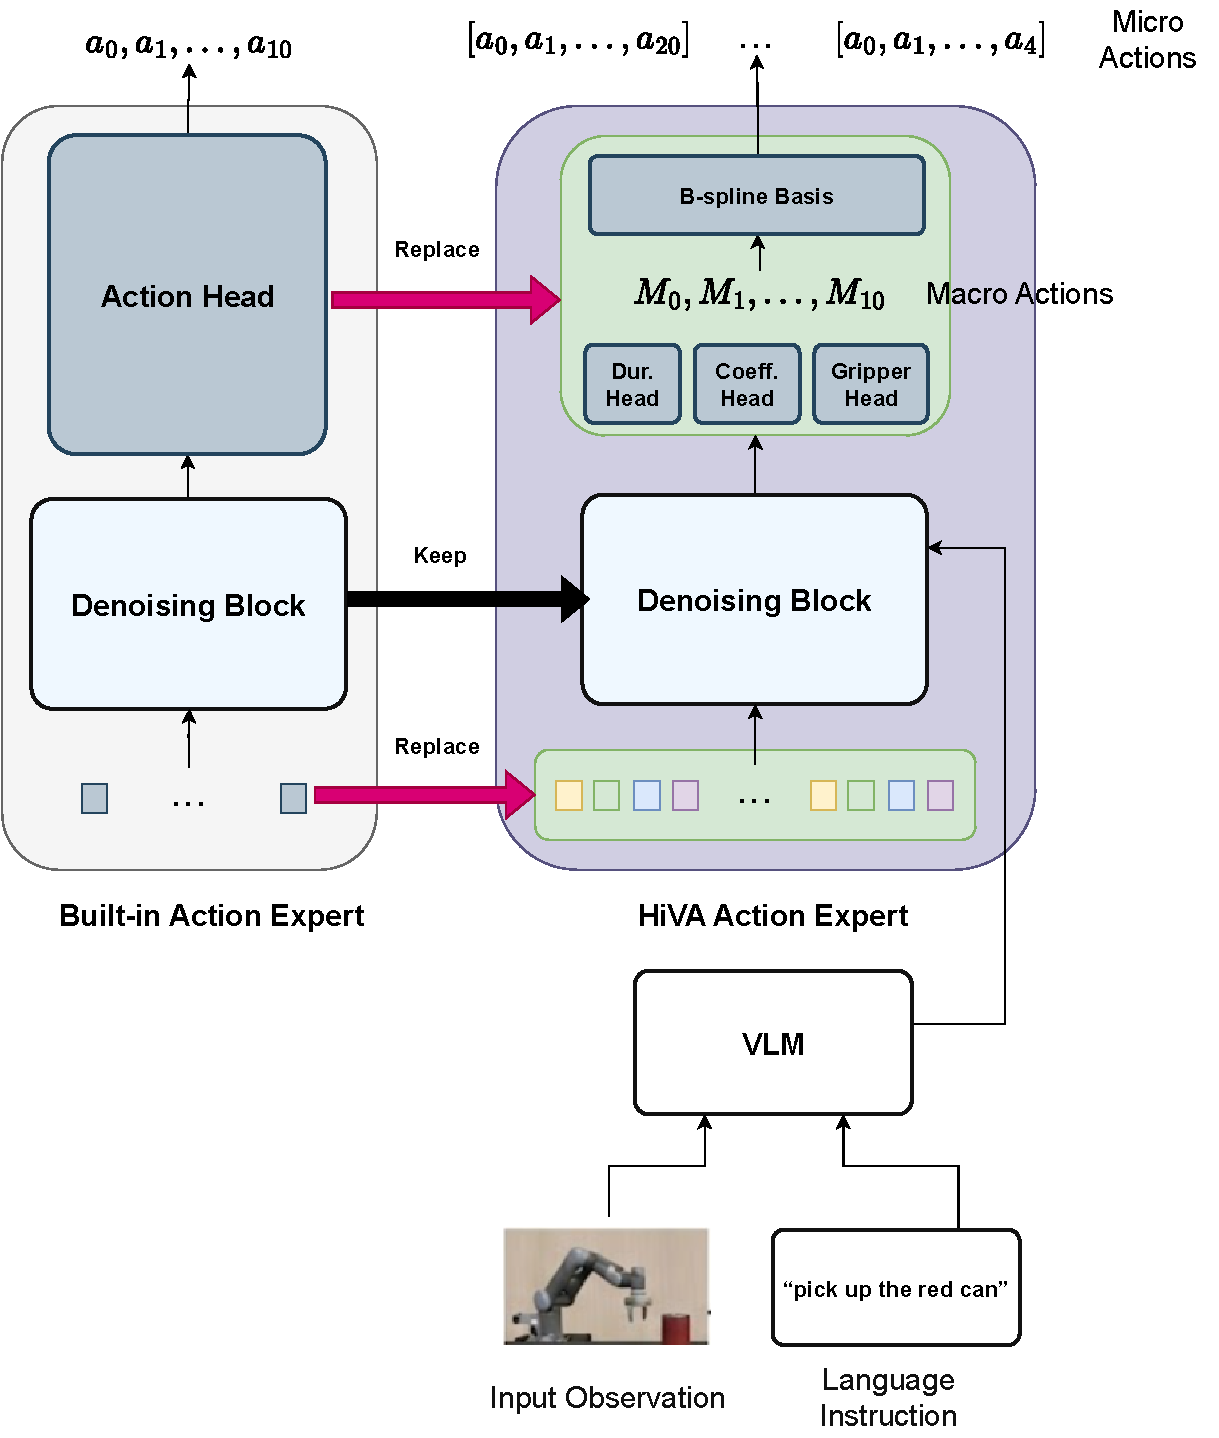
\includegraphics[width=\linewidth]{HiVA_architecture.pdf}
    \caption{HiVA architecture. HiVA replaces the fixed raw-action interface of a denoising VLA action expert with a macro-action interface. The action tokens are decomposed into duration, translation-coefficient, rotation-coefficient, and gripper tokens, allowing each macro action to capture both a behavioral segment and fine-grained control within that segment. The built-in action head is replaced by duration, coefficient, and gripper heads, and a B-spline basis converts the predicted coefficients and duration into smooth variable-length micro-actions.}
    \label{fig:hiva-architecture}
\end{figure}

\Cref{fig:hiva-architecture} shows how HiVA is inserted into a denoising-based VLA. Instead of asking the action expert to predict a fixed horizon of raw micro-actions, we replace the action-token interface with macro-action tokens: a duration token that determines the number of micro-steps, translation and rotation coefficient tokens that describe smooth cumulative motion, and gripper coefficient tokens that describe the continuous absolute gripper command. The corresponding output heads produce a macro action, and the B-spline basis expands the duration-conditioned coefficients into the final micro-action sequence. This design lets a single macro action represent a meaningful behavioral segment, while still preserving fine-grained translation, rotation, and gripper control inside that segment.

To make the approach easy to integrate into existing denoising-based VLAs, we only change a small number of lightweight layers and heads outside the main denoising transformer block in the action expert. Specifically, as summarized in \cref{fig:hiva-architecture}, we keep the pretrained multimodal conditioning path and the main denoising transformer intact, and replace only the early action-side projection layers and the output heads. We instantiate this design in SmolVLA and VPP \cite{smolvla2025,vpp2024}. In both cases, the raw fixed-horizon action interface is replaced by duration, coefficient, and gripper heads while the main pretrained denoising transformer remains unchanged.

\subsection{Macro-action parameterization}
For translation and rotation, the action expert predicts cubic B-spline coefficients in a chunk-relative cumulative representation. Let $\Phi_{d_j}\in\mathbb{R}^{d_j\times K}$ denote the cubic B-spline basis matrix for duration $d_j$. Translation is reconstructed as
\begin{equation}
\hat P_j = \Phi_{d_j}\Theta^{\mathrm{tr}}_j,
\end{equation}
where $\hat P_j(\tau)$ is the cumulative translation from the start of the chunk to local micro-step $\tau$. Rotation is reconstructed similarly,
\begin{equation}
\hat R_j = \Phi_{d_j}\Theta^{\mathrm{rot}}_j,
\end{equation}
where $\hat R_j(\tau)$ is the cumulative rotation vector relative to the chunk start.

The gripper is represented with B-spline coefficients over the native continuous command. In LIBERO-style end-effector control, the final action dimension is an absolute command $g_t\in[-1,1]$ rather than a delta. Therefore we do not integrate or cumulative-sum gripper values. For duration $d_j$, let $\Phi^{\mathrm{grip}}_{d_j}\in\mathbb{R}^{d_j\times K_g}$ denote the gripper basis. The decoded gripper sequence is
\begin{equation}
\hat G_j=\Phi^{\mathrm{grip}}_{d_j}\Theta_j^{\mathrm{grip}},
\qquad
\hat G_j(\tau)\in[-1,1].
\end{equation}
The first coding experiments use the same cubic basis for translation, rotation, and gripper so the implementation has one coefficient-token pattern. A binary event/switch-time gripper head remains a secondary Plan-B design.

\subsection{Joint duration reasoning with a denoising action expert}
Duration and coefficients are reasoned jointly by the same transformer block, but they use different output types. The duration token is supervised with a bounded discrete head over $\{1,\dots,D_{\max}\}$, while coefficient tokens are optimized with a continuous denoising objective, instantiated as flow matching or diffusion denoising depending on the host action expert. This design lets duration and coefficients interact through self-attention without forcing a discrete variable into the same continuous objective.

During training, the predicted duration distribution also participates in a soft duration-aware reconstruction. Instead of selecting a single hard predicted duration, we form a weighted mixture over hold-padded B-spline bases, so duration errors directly affect the reconstructed cumulative trajectories. This gives the model a clean way to learn that underestimating duration flattens a chunk too early, while overestimating duration causes unnecessary motion after the ground-truth chunk ends.

\subsection{Compact training objective}
Let $J$ be the number of macro tokens in a training sample. The total loss is
\begin{equation}
L_{\text{total}} = \frac{1}{J}\sum_{j=1}^{J} L_j,
\end{equation}
with
\begin{align}
L_j =\;& \lambda_{\mathrm{dur}}L_{\mathrm{dur},j}
+ \lambda_{\mathrm{den}}^{\mathrm{tr}}L_{\mathrm{den},j}^{\mathrm{tr}}
+ \lambda_{\mathrm{path}}^{\mathrm{tr}}L_{\mathrm{path},j}^{\mathrm{tr}} \nonumber\\
&+ \lambda_{\mathrm{tail}}^{\mathrm{tr}}L_{\mathrm{tail},j}^{\mathrm{tr}}
+ \lambda_{\mathrm{den}}^{\mathrm{rot}}L_{\mathrm{den},j}^{\mathrm{rot}}
+ \lambda_{\mathrm{path}}^{\mathrm{rot}}L_{\mathrm{path},j}^{\mathrm{rot}} \nonumber\\
&+ \lambda_{\mathrm{tail}}^{\mathrm{rot}}L_{\mathrm{tail},j}^{\mathrm{rot}}
+ \lambda_{\mathrm{den}}^{\mathrm{grip}}L_{\mathrm{den},j}^{\mathrm{grip}} \nonumber\\
&+ \lambda_{\mathrm{path}}^{\mathrm{grip}}L_{\mathrm{path},j}^{\mathrm{grip}}
+ \lambda_{\mathrm{tail}}^{\mathrm{grip}}L_{\mathrm{tail},j}^{\mathrm{grip}}.
\label{eq:total-loss-main}
\end{align}
Here $L_{\mathrm{dur}}$ supervises the duration categorical distribution. The denoising losses $L_{\mathrm{den}}^{\mathrm{tr}}$, $L_{\mathrm{den}}^{\mathrm{rot}}$, and $L_{\mathrm{den}}^{\mathrm{grip}}$ supervise translation, rotation, and gripper coefficients in the host continuous denoising objective. The path and tail losses measure decoded reconstruction error on the valid chunk prefix and the hold-padded suffix. Detailed definitions and simplified pilot variants are provided in the appendix.

\section{Training Dataset and Evaluation Benchmarks}
\subsection{Training dataset construction}
We relabel each expert trajectory into macro-actions with a dynamic-programming (DP) oracle. Consider a candidate segment that starts at micro-step $s$ and spans $d$ micro-actions. Its cost is
\begin{equation}
C_{s,d} = \gamma + \alpha E_{s,d} + \beta R^{\mathrm{evt}}_{s,d},
\label{eq:segment-cost}
\end{equation}
where $E_{s,d}$ is a B-spline fit error and $R^{\mathrm{evt}}_{s,d}$ is an event-proximity risk.

For a candidate segment, we construct chunk-relative cumulative translation and rotation targets in the native command space of the expert trajectory. In LIBERO, the raw action is
\begin{equation}
a_t = [\Delta x_t,\Delta y_t,\Delta z_t,
       \Delta r^x_t,\Delta r^y_t,\Delta r^z_t,g_t],
\end{equation}
where the first three entries are relative translation commands, the next three entries are relative rotation-vector commands, and $g_t$ is an absolute continuous gripper command. The cumulative translation target for local index $\tau\in\{1,\dots,d\}$ is
\begin{equation}
P^{\star}_{s,d}(\tau) = \sum_{m=1}^{\tau}a^\star_{s+m-1}[0:3].
\end{equation}
The cumulative rotation target is obtained by composing the commanded rotation-vector deltas in $SO(3)$. If $\eta$ is the controller scale from raw action units to radians, $\eta=0.5$ for the LIBERO OSC\_POSE configuration used here, then
\begin{equation}
\mathcal{R}_{s,d}^{\star}(0)=I,
\qquad
\mathcal{R}_{s,d}^{\star}(\tau)=
\mathcal{R}_{s,d}^{\star}(\tau-1)
\operatorname{Exp}\!\left(\eta\,a^\star_{s+\tau-1}[3:6]\right),
\end{equation}
with
\begin{equation}
R^{\star}_{s,d}(\tau)=
\operatorname{Log}\!\left(\mathcal{R}_{s,d}^{\star}(\tau)\right)
\in\mathbb{R}^3.
\end{equation}
Thus the spline is fit to cumulative command-space axis vectors, and native relative rotation-vector actions are recovered at decode time by adjacent $SO(3)$ differences. The gripper target is the original absolute command sequence, not a cumulative sum. A cubic B-spline is then fit to each candidate segment by regularized least squares, and the fit error is computed from the resulting reconstruction error.

To discourage macro-actions from crossing delicate event boundaries, we define a per-step event risk. Let $e_i$ and $e_{i+1}$ denote two consecutive gripper event times, and let $L_i=e_{i+1}-e_i$. For a micro-step $u$ with $e_i\le u < e_{i+1}$, we define a normalized pre-event term
\begin{equation}
r^{\mathrm{pre}}_{u,i} =
\frac{\alpha_{\mathrm{pre}}}
{\frac{(e_{i+1}-1)-u}{\max(1,L_i-1)}+\delta},
\end{equation}
and a delayed post-event bump
\begin{equation}
r^{\mathrm{post},\rho}_{u,i} =
\alpha_{\mathrm{post}}\,\mathbf{1}[u\ge e_i+\rho]
\exp\!\left(-\frac{u-(e_i+\rho)}{\tau_{\mathrm{post}}}\right),
\end{equation}
with $\tau_{\mathrm{post}}=2$. The segment-level event risk is aggregated with log-sum-exp:
\begin{equation}
R^{\mathrm{evt}}_{s,d} = \frac{1}{\kappa}
\log\sum_{u=s}^{s+d-1}\exp\bigl(\kappa(r^{\mathrm{pre}}_{u,i(u)}+r^{\mathrm{post},\rho}_{u,i(u)})\bigr),
\end{equation}
where $i(u)$ is the most recent gripper event index such that $e_{i(u)}\le u$.

We impose the gripper rule as a separate hard feasibility constraint rather than folding it into the cost. Let $\nu_{s,d}$ be the number of gripper flips in the candidate segment and let $\ell_{s,d}$ be the number of micro-steps after the first flip inside the same segment. Then the candidate is infeasible when
\begin{equation}
\nu_{s,d}>1 \quad \text{or} \quad \ell_{s,d}>\rho,
\end{equation}
and we set
\begin{equation}
C_{s,d}=+\infty.
\end{equation}
This ensures that each macro-action contains at most one gripper event and at most $\rho$ settle steps after that event.

The optimal segmentation is obtained by dynamic programming:
\begin{equation}
F[0]=0, \qquad
F[t]=\min_{d\in\mathcal{D},\,d\le t}\bigl(F[t-d]+C_{t-d+1,d}\bigr).
\label{eq:dp}
\end{equation}
Backtracking from $F[T]$ yields the final macro boundaries and therefore the GT duration labels $d_j^{\star}$. For each selected segment, we retain the fitted translation and rotation coefficients, the cumulative translation and rotation targets, the binary gripper sequence, the gripper start state, and the event/timing labels used by the action expert.

\subsection{Benchmarks}
We use two long-horizon manipulation benchmarks. LIBERO-Plus extends the original LIBERO benchmark with controlled perturbations over object layout, camera viewpoint, robot initial state, language, lighting, background, and sensor noise, exposing substantially lower and more diagnostic performance for existing VLA models than the original LIBERO suites \cite{libero2023,liberoplus2025}. We therefore target LIBERO-Plus rather than the original LIBERO benchmark to stress-test robustness under realistic distribution shifts. CALVIN is explicitly designed for long-horizon language-conditioned manipulation and is commonly evaluated by the average number of chained tasks completed successfully in sequence \cite{calvin2021}. We use LIBERO-Plus and CALVIN because both require the policy to maintain consistency across multi-phase manipulation sequences rather than solve isolated one-step reactions.

\subsection{Backbones and protocol}
We evaluate the proposed action expert in two representative denoising-based VLAs with different model-size scales: SmolVLA (0.45B) and VPP (1.5B) \cite{smolvla2025,vpp2024}. In both cases, we keep the main pretrained denoising transformer block and the multimodal conditioning path, and replace only the small action-side layers surrounding that block. SmolVLA is evaluated on LIBERO-Plus, while VPP is evaluated on CALVIN.

The main comparisons are against the original raw-action experts of the host architectures. For LIBERO-Plus, we compare SmolVLA against SmolVLA+HiVA(ours), using the existing SmolVLA task-success baseline of 69.0\% as the reference. For CALVIN, we compare VPP against VPP+HiVA(ours), using the existing VPP average completed sequence length of 4.33 in the full-data setting and 3.25 in the data-efficiency setting as references. We will also report the number of model calls per episode and total completion time to measure whether variable-length macro-actions reduce inference cost while preserving or improving success.

\appendix

\section{Detailed Training Objective}
\label{app:training-objective}
This appendix expands the compact loss in \cref{eq:total-loss-main}. Throughout the appendix, $D_{\max}$ is the maximum macro duration and $K$ is the number of spline basis functions.


\subsection{Command-space cumulative axis-vector rotation labels}
\label{app:liberoplus-rotation}
The implementation does not use observed end-effector quaternion displacement as the primary rotation label. That diagnostic target was geometrically meaningful as a state trajectory, but it introduced a large gap between the original LIBERO rotation-vector command sequence and the rotation deltas reconstructed from fitted B-spline coefficients. HiVA therefore uses \emph{command-space cumulative rotation}: the spline is fit to cumulative axis vectors obtained by composing the native relative rotation-vector action commands.

Let the raw LIBERO action be
\begin{equation}
a_t = [\Delta x_t,\Delta y_t,\Delta z_t,
       \Delta r^x_t,\Delta r^y_t,\Delta r^z_t,g_t],
\end{equation}
where $a_t[3:6]$ is a relative rotation-vector command and $g_t\in[-1,1]$ is an absolute gripper command. Let $\eta>0$ denote the controller scale from raw action units to radians; in the current LIBERO OSC\_POSE setup we use $\eta=0.5$. For a candidate segment starting at frame $s$, define
\begin{equation}
\Delta R_{s+\tau-1}^{\star}
=
\operatorname{Exp}\!\left(\eta\,a^\star_{s+\tau-1}[3:6]\right),
\qquad
\tau=1,\ldots,d.
\end{equation}
The cumulative command-space rotation is composed on $SO(3)$:
\begin{equation}
\mathcal{R}_{s}^{\star}(0)=I,
\qquad
\mathcal{R}_{s}^{\star}(\tau)=
\mathcal{R}_{s}^{\star}(\tau-1)
\Delta R_{s+\tau-1}^{\star}.
\end{equation}
The cumulative axis-vector label used for B-spline fitting is
\begin{equation}
\rho_s^{\star}(\tau)=
\operatorname{Log}\!\left(\mathcal{R}_{s}^{\star}(\tau)\right)
\in\mathbb{R}^3,
\qquad
\tau=1,\ldots,d.
\end{equation}
For a duration-specific basis $\Phi_d$, the offline coefficient target solves
\begin{equation}
\Theta_{s,\mathrm{rot}}^{\star}
=
\arg\min_{\Theta\in\mathbb{R}^{K\times3}}
\left\|\Phi_d\Theta-\rho_s^{\star}\right\|_2^2
+\lambda_{\mathrm{ridge}}\|\Theta\|_F^2.
\end{equation}
For the canonical hold-pad experiment in \cref{app:exp-hp-hiva}, the same cumulative axis-vector prefix is first hold-padded to $D_{\max}$ and then fit with the single canonical basis $\Phi_{D_{\max}}$.

At inference, the model predicts raw rotation coefficients $\hat\Theta^{\mathrm{rot}}$ after coefficient unnormalization. A basis matrix $\Phi$ decodes cumulative axis vectors
\begin{equation}
\hat\rho(\tau)=\Phi(\tau,:)\hat\Theta^{\mathrm{rot}}.
\end{equation}
These cumulative axis vectors are converted back to native relative rotation-vector actions by adjacent differences on $SO(3)$:
\begin{equation}
\hat{\mathcal{R}}(\tau)=\operatorname{Exp}\!\left(\hat\rho(\tau)\right),
\qquad
\Delta\hat{\mathcal{R}}(\tau)=
\hat{\mathcal{R}}(\tau-1)^{-1}\hat{\mathcal{R}}(\tau),
\end{equation}
with $\hat{\mathcal{R}}(0)=I$. The reconstructed native LIBERO rotation-vector command is
\begin{equation}
\hat a^{\mathrm{rot}}_{s+\tau-1}
=
\frac{1}{\eta}
\operatorname{Log}\!\left(\Delta\hat{\mathcal{R}}(\tau)\right).
\end{equation}
This construction makes the fitted target and the executed action live in the same command space. The only approximation is the B-spline reconstruction error, not an implicit inversion of observed controller dynamics.

\subsection{Duration loss}
Let the duration token produce logits
\begin{equation}
z_j^{\mathrm{dur}} = W_{\mathrm{dur}} h_j^{\mathrm{dur}} \in \mathbb{R}^{D_{\max}}.
\end{equation}
The duration distribution is
\begin{equation}
\pi_{j,d}=\operatorname{softmax}(z_j^{\mathrm{dur}})_d,
\qquad d\in\{1,\dots,D_{\max}\}.
\end{equation}
The duration loss is cross-entropy plus an ordinal penalty:
\begin{equation}
L_{\mathrm{dur},j} = -\log\pi_{j,d_j^{\star}} + \lambda_{\mathrm{ord}}
\sum_{d=1}^{D_{\max}} \pi_{j,d}
\left(\frac{d-d_j^{\star}}{D_{\max}-1}\right)^2.
\end{equation}

\subsection{Soft duration-aware reconstruction}
For each duration $d$, let $\Phi_d\in\mathbb{R}^{d\times K}$ be the cubic B-spline basis matrix. To make all candidate durations compatible inside one fixed-size tensor, we define a hold-padded basis matrix $\widetilde\Phi_d^{\mathrm{hold}}\in\mathbb{R}^{D_{\max}\times K}$ by
\begin{equation}
\widetilde\Phi_d^{\mathrm{hold}}(\tau,:)=
\begin{cases}
\Phi_d(\tau,:), & \tau\le d,\\
\Phi_d(d,:), & \tau>d.
\end{cases}
\end{equation}
The soft duration-aware basis mixture is then
\begin{equation}
\bar\Phi_j = \sum_{d=1}^{D_{\max}} \pi_{j,d}\,\widetilde\Phi_d^{\mathrm{hold}}.
\end{equation}
Let $\hat\Theta_j^{\mathrm{tr}},\hat\Theta_j^{\mathrm{rot}}\in\mathbb{R}^{K\times 3}$ denote the predicted translation and rotation coefficients. The reconstructed cumulative trajectories are
\begin{equation}
\hat P_j = \bar\Phi_j\hat\Theta_j^{\mathrm{tr}},
\qquad
\hat R_j = \bar\Phi_j\hat\Theta_j^{\mathrm{rot}}.
\end{equation}

For a GT macro duration $d_j^{\star}$, define hold-padded cumulative GT targets
\begin{equation}
\widetilde P_j^{\star}(\tau)=
\begin{cases}
P_j^{\star}(\tau), & \tau\le d_j^{\star},\\
P_j^{\star}(d_j^{\star}), & \tau>d_j^{\star},
\end{cases}
\end{equation}
\begin{equation}
\widetilde R_j^{\star}(\tau)=
\begin{cases}
R_j^{\star}(\tau), & \tau\le d_j^{\star},\\
R_j^{\star}(d_j^{\star}), & \tau>d_j^{\star}.
\end{cases}
\end{equation}
Let $m_{j,\tau}=\mathbf{1}[\tau\le d_j^{\star}]$ and $M_j=m_j\mathbf{1}_3^\top$. Then
\begin{equation}
L_{\mathrm{path},j}^{\mathrm{tr}} = \frac{1}{d_j^{\star}}
\left\|M_j\odot(\hat P_j-\widetilde P_j^{\star})\right\|_1,
\end{equation}
\begin{equation}
L_{\mathrm{tail},j}^{\mathrm{tr}} = \frac{1}{\max(1,D_{\max}-d_j^{\star})}
\left\|(1-M_j)\odot(\hat P_j-\widetilde P_j^{\star})\right\|_1.
\end{equation}
The rotation path and tail losses are defined analogously:
\begin{equation}
L_{\mathrm{path},j}^{\mathrm{rot}} = \frac{1}{d_j^{\star}}
\left\|M_j\odot(\hat R_j-\widetilde R_j^{\star})\right\|_1,
\end{equation}
\begin{equation}
L_{\mathrm{tail},j}^{\mathrm{rot}} = \frac{1}{\max(1,D_{\max}-d_j^{\star})}
\left\|(1-M_j)\odot(\hat R_j-\widetilde R_j^{\star})\right\|_1.
\end{equation}

\subsection{Continuous denoising objective for translation and rotation coefficients}
The coefficient branch uses the native continuous denoising objective of the host action expert. We therefore write the main translation and rotation losses in the generic form $L_{\mathrm{den},j}^{\mathrm{tr}}$ and $L_{\mathrm{den},j}^{\mathrm{rot}}$.

\paragraph{Flow-matching instantiation.}
For flow-matching backbones, let $\Theta_j^{\mathrm{tr},\star}$ be the GT translation coefficient matrix and sample $u\sim\mathcal{U}[0,1]$, $\epsilon_j^{\mathrm{tr}}\sim\mathcal{N}(0,I)$. Define
\begin{equation}
\Theta_j^{\mathrm{tr},u} = u\Theta_j^{\mathrm{tr},\star} + (1-u)\epsilon_j^{\mathrm{tr}},
\end{equation}
and use the vector-field objective
\begin{equation}
L_{\mathrm{den},j}^{\mathrm{tr}} =
\mathbb{E}_{u,\epsilon_j^{\mathrm{tr}}}
\left[\left\|v_{\theta}^{\mathrm{tr}}(\Theta_j^{\mathrm{tr},u},u,c_j)-\bigl(\epsilon_j^{\mathrm{tr}}-\Theta_j^{\mathrm{tr},\star}\bigr)\right\|_F^2\right].
\end{equation}
The rotation version is identical with the superscript \texttt{rot}.

\paragraph{Diffusion instantiation.}
For diffusion backbones, one may instead sample a noise level $t$ with cumulative schedule $\bar\alpha_t$ and define
\begin{equation}
\Theta_j^{\mathrm{tr},t} = \sqrt{\bar\alpha_t}\,\Theta_j^{\mathrm{tr},\star} + \sqrt{1-\bar\alpha_t}\,\epsilon_j^{\mathrm{tr}}.
\end{equation}
The translation denoising loss becomes
\begin{equation}
L_{\mathrm{den},j}^{\mathrm{tr}} =
\mathbb{E}_{t,\epsilon_j^{\mathrm{tr}}}
\left[\left\|\epsilon_{\theta}^{\mathrm{tr}}(\Theta_j^{\mathrm{tr},t},t,c_j)-\epsilon_j^{\mathrm{tr}}\right\|_F^2\right],
\end{equation}
with the analogous rotation objective.

\subsection{Plan-B gripper event heads and reconstruction}
We use a binary gripper event space $\{\texttt{hold},\texttt{flip}\}$. Let the gripper token produce event logits
\begin{equation}
z_j^{\mathrm{evt}} = W_{\mathrm{evt}}h_j^{\mathrm{grip}} \in \mathbb{R}^{2},
\end{equation}
with distribution
\begin{equation}
p_j^{\mathrm{evt}} = \operatorname{softmax}(z_j^{\mathrm{evt}}).
\end{equation}
The event loss is
\begin{equation}
L_{\mathrm{evt},j} = -\log p_j^{\mathrm{evt}}(e_j^{\star}).
\end{equation}

For switch time, let
\begin{equation}
z_j^{\mathrm{time}} = W_{\mathrm{time}}h_j^{\mathrm{grip}} \in \mathbb{R}^{D_{\max}}.
\end{equation}
During training, mask logits beyond the GT duration:
\begin{equation}
\widetilde z_{j,\tau}^{\mathrm{time}} =
\begin{cases}
z_{j,\tau}^{\mathrm{time}}, & \tau\le d_j^{\star},\\
-\infty, & \tau>d_j^{\star}.
\end{cases}
\end{equation}
Then
\begin{equation}
p_j^{\mathrm{time}} = \operatorname{softmax}(\widetilde z_j^{\mathrm{time}}),
\qquad
C_{j,\tau}=\sum_{m=1}^{\tau}p_j^{\mathrm{time}}(m).
\end{equation}
The switch-time loss is defined only when the GT event is \texttt{flip}:
\begin{equation}
L_{\mathrm{time},j} = \mathbf{1}[e_j^{\star}=\texttt{flip}]\,\bigl(-\log p_j^{\mathrm{time}}(\tau_j^{\star})\bigr).
\end{equation}

Let $g_j^{\mathrm{start}}\in\{0,1\}$ be the gripper state at the start of macro $j$. During training we use the GT start state; during inference we use the observed current state for the first macro and the previous predicted final state for later macros. The predicted probability that the gripper is open at local micro-step $\tau$ is
\begin{align}
\hat g_{j,\tau}^{\mathrm{open}}
=\;& p_j^{\mathrm{evt}}(\texttt{hold})\,g_j^{\mathrm{start}} \nonumber\\
&+ p_j^{\mathrm{evt}}(\texttt{flip})\,g_j^{\mathrm{start}}(1-C_{j,\tau}) \nonumber\\
&+ p_j^{\mathrm{evt}}(\texttt{flip})\,(1-g_j^{\mathrm{start}})\,C_{j,\tau}.
\end{align}

Let the GT binary gripper sequence in macro $j$ be $g_j^{\star}(1),\dots,g_j^{\star}(d_j^{\star})$. Hold-pad it by terminal extension:
\begin{equation}
\widetilde g_j^{\star}(\tau)=
\begin{cases}
g_j^{\star}(\tau), & \tau\le d_j^{\star},\\
g_j^{\star}(d_j^{\star}), & \tau>d_j^{\star}.
\end{cases}
\end{equation}
Then the gripper path and tail losses are
\begin{equation}
L_{\mathrm{path},j}^{\mathrm{grip}} =
\frac{1}{d_j^{\star}}\sum_{\tau=1}^{d_j^{\star}}
\operatorname{BCE}\bigl(\hat g_{j,\tau}^{\mathrm{open}},\widetilde g_j^{\star}(\tau)\bigr),
\end{equation}
\begin{equation}
L_{\mathrm{tail},j}^{\mathrm{grip}} =
\frac{1}{\max(1,D_{\max}-d_j^{\star})}\sum_{\tau=d_j^{\star}+1}^{D_{\max}}
\operatorname{BCE}\bigl(\hat g_{j,\tau}^{\mathrm{open}},\widetilde g_j^{\star}(\tau)\bigr).
\end{equation}

\subsection{Complete macro loss}
Combining all parts yields the loss quoted in the main paper:
\begin{align}
L_j =\;& \lambda_{\mathrm{dur}}L_{\mathrm{dur},j}
+ \lambda_{\mathrm{den}}^{\mathrm{tr}}L_{\mathrm{den},j}^{\mathrm{tr}} \nonumber\\
&+ \lambda_{\mathrm{path}}^{\mathrm{tr}}L_{\mathrm{path},j}^{\mathrm{tr}}
+ \lambda_{\mathrm{tail}}^{\mathrm{tr}}L_{\mathrm{tail},j}^{\mathrm{tr}} \nonumber\\
&+ \lambda_{\mathrm{den}}^{\mathrm{rot}}L_{\mathrm{den},j}^{\mathrm{rot}}
+ \lambda_{\mathrm{path}}^{\mathrm{rot}}L_{\mathrm{path},j}^{\mathrm{rot}} \nonumber\\
&+ \lambda_{\mathrm{tail}}^{\mathrm{rot}}L_{\mathrm{tail},j}^{\mathrm{rot}}
+ \lambda_{\mathrm{den}}^{\mathrm{grip}}L_{\mathrm{den},j}^{\mathrm{grip}} \nonumber\\
&+ \lambda_{\mathrm{path}}^{\mathrm{grip}}L_{\mathrm{path},j}^{\mathrm{grip}}
+ \lambda_{\mathrm{tail}}^{\mathrm{grip}}L_{\mathrm{tail},j}^{\mathrm{grip}}.
\end{align}


\section{Preliminary HiVA-Lite Experiments}
\label{app:prelim-hiva-lite}
This appendix records the simplified first experiments used before the full DP-based HiVA system. The goal is to produce an interpretable preliminary result on LIBERO with minimal changes to SmolVLA: the model learns when to execute short, medium, or long prefixes, while the original raw action chunk training path remains largely unchanged.

\subsection{Experiment 1: duration-only SmolVLA}
\label{app:exp-duration-only}
The first experiment keeps SmolVLA's raw action representation but adds a true duration token to the action expert. The suffix sequence processed by the SmolVLA denoising expert therefore contains the original $N=50$ action tokens plus one additional learned duration token. This duration token passes through the same denoising attention layers as the action suffix tokens and is decoded by a lightweight categorical duration head. Let the duration set be
\begin{equation}
\mathcal{D}=\{1,3,8\}.
\end{equation}
Given observation $o_s$, language instruction $\ell$, and the host SmolVLA action expert, the model predicts an $N$-step raw action chunk
\begin{equation}
\hat A_s=(\hat a_s,\hat a_{s+1},\ldots,\hat a_{s+N-1})\in\mathbb{R}^{N\times 7}
\end{equation}
from the action-token outputs, and duration logits
\begin{equation}
z_s^{\mathrm{dur}}\in\mathbb{R}^{3},
\qquad
\pi_s=\operatorname{softmax}(z_s^{\mathrm{dur}}),
\end{equation}
from the duration-token output. The duration logits are not produced by mean-pooling the action tokens; the duration token is its own suffix token and has its own hidden state after the expert attention stack. The three classes correspond to durations $[1,3,8]$.

The duration label $d_s^\star$ is a dense per-frame horizon label from the sidecar dataset rather than a non-overlapping DP macro label. In the current LIBERO pilot, the sidecar labeler combines explicit gripper switch zones with saved pure-contact-frame annotations and assigns the conservative horizon-safe target at each possible training start $s$. Thus, Experiment 1 tests whether the model can learn when to execute short, medium, or long prefixes without changing the underlying action representation.

During training, the original $N$-action flow-matching loss is retained. The duration head is supervised with a clean teacher-forced suffix pass: the ground-truth clean action chunk $A_s^\star$ is embedded with timestep $t=0$, the learned duration token is appended after the $N$ action tokens, and the resulting duration-token hidden state produces $z_s^{\mathrm{dur}}$. The total loss is
\begin{equation}
L_{\mathrm{total}} = L_{\text{FM-action}}
+ \lambda_{\mathrm{dur}}\left[-\log \pi_s(d_s^{\star})\right].
\label{eq:prelim-duration-loss}
\end{equation}
At inference, SmolVLA first denoises the full raw action chunk as usual. A final clean $t=0$ suffix pass embeds the denoised action chunk together with the duration token and predicts
\begin{equation}
\hat d_s = \arg\max_{d\in\mathcal{D}}\pi_s(d),
\end{equation}
after which the controller executes only the first $\hat d_s$ actions from the predicted raw chunk before re-observing:
\begin{equation}
\hat a_s,\hat a_{s+1},\ldots,\hat a_{s+\hat d_s-1}.
\end{equation}
Thus $N$ is still the raw training and prediction chunk length, while $\hat d_s$ is the executed prefix length. Evaluation is kept at batch size one so each environment can use its own predicted execution horizon.

\subsection{Experiment 2: one-macro translation-coefficient HiVA-lite}
\label{app:exp-one-macro-trans}
The second preliminary experiment introduces a one-macro translation coefficient head while keeping rotation and gripper prediction in the regular SmolVLA raw action stream. Let $\mathcal{D}=\{1,3,8\}$, let $D_{\max}=\max\mathcal{D}=8$, and let $K_{\max}=4$. The model predicts three outputs: an $N$-step raw action chunk $\hat A_s^{\mathrm{raw}}$, a duration distribution $\pi_s$, and translation coefficients $\hat\Theta_s^{\mathrm{tr}}\in\mathbb{R}^{K_{\max}\times 3}$. For each $d\in\mathcal{D}$, let $\bar\Phi_d\in\mathbb{R}^{D_{\max}\times K_{\max}}$ denote the padded translation basis matrix: if $K(d)<K_{\max}$, unused columns are zero-padded, and for rows $\tau>d$ the final cumulative row is repeated so the decoded translation holds after duration $d$. The soft duration-aware mixed basis is
\begin{equation}
\bar\Phi_s^{\mathrm{mix}}=
\sum_{d\in\mathcal{D}}\pi_s(d)\,\bar\Phi_d.
\end{equation}
The cumulative translation trajectory for the first $D_{\max}$ steps is then
\begin{equation}
\hat P_s^{\mathrm{tr}}=
\bar\Phi_s^{\mathrm{mix}}\hat\Theta_s^{\mathrm{tr}}
\in\mathbb{R}^{D_{\max}\times 3},
\end{equation}
and the decoded translation micro-actions are obtained by finite differences,
\begin{equation}
\begin{aligned}
\hat u_{s+\tau-1}^{\mathrm{tr,coef}}
&=\hat P_s^{\mathrm{tr}}(\tau)-\hat P_s^{\mathrm{tr}}(\tau-1),\\
\tau&=1,\ldots,D_{\max},
\qquad \hat P_s^{\mathrm{tr}}(0)=0.
\end{aligned}
\end{equation}
Let $\hat A_s^{\mathrm{raw}}=(\hat a_s^{\mathrm{raw}},\ldots,\hat a_{s+N-1}^{\mathrm{raw}})$, where each raw action is decomposed as
\begin{equation}
\hat a_{s+\tau-1}^{\mathrm{raw}}=
\left[
\hat u_{s+\tau-1}^{\mathrm{tr,raw}},
\hat u_{s+\tau-1}^{\mathrm{rot,raw}},
\hat u_{s+\tau-1}^{\mathrm{grip,raw}}
\right].
\end{equation}
During training, the assembled predicted action chunk $\bar A_s=(\bar a_s,\ldots,\bar a_{s+N-1})$ uses coefficient-decoded translation on the first $D_{\max}$ tokens and the raw SmolVLA prediction afterwards. Define
\begin{equation}
\hat a_{s+\tau-1}^{\mathrm{coef}}=
\left[
\hat u_{s+\tau-1}^{\mathrm{tr,coef}},
\hat u_{s+\tau-1}^{\mathrm{rot,raw}},
\hat u_{s+\tau-1}^{\mathrm{grip,raw}}
\right].
\end{equation}
Then
\begin{equation}
\bar a_{s+\tau-1}=
\begin{cases}
\hat a_{s+\tau-1}^{\mathrm{coef}}, & 1\le \tau\le D_{\max},\\[4pt]
\hat a_{s+\tau-1}^{\mathrm{raw}}, & D_{\max}<\tau\le N.
\end{cases}
\end{equation}
For the GT duration $d_s^{\star}$, define the GT cumulative translation prefix
\begin{equation}
P_s^{\star}(\tau)=
\sum_{m=1}^{\tau}u_{s+m-1}^{\mathrm{tr},\star},
\qquad
\tau=1,\ldots,d_s^{\star},
\end{equation}
then hold-pad it to $D_{\max}$ by
\begin{equation}
\widetilde P_s^{\star}(\tau)=
\begin{cases}
P_s^{\star}(\tau), & \tau\le d_s^{\star},\\
P_s^{\star}(d_s^{\star}), & d_s^{\star}<\tau\le D_{\max},
\end{cases}
\qquad
\widetilde P_s^{\star}(0)=0.
\end{equation}
The hold-padded GT translation micro-actions for the first $D_{\max}$ steps are
\begin{equation}
\widetilde u_{s+\tau-1}^{\mathrm{tr},\star}=
\widetilde P_s^{\star}(\tau)-\widetilde P_s^{\star}(\tau-1),
\qquad
\tau=1,\ldots,D_{\max}.
\end{equation}
The hybrid GT target chunk $\widetilde A_s^{\star}=(\widetilde a_s^{\star},\ldots,\widetilde a_{s+N-1}^{\star})$ uses the padded GT translation for the first $D_{\max}$ tokens, the original GT translation from $D_{\max}+1$ to $N$, and the GT rotation/gripper for all action tokens:
\begin{equation}
\widetilde a_{s+\tau-1}^{\star}=
\begin{cases}
\left[
\widetilde u_{s+\tau-1}^{\mathrm{tr},\star},
 u_{s+\tau-1}^{\mathrm{rot},\star},
 u_{s+\tau-1}^{\mathrm{grip},\star}
\right], & 1\le \tau\le D_{\max},\\[4pt]
a_{s+\tau-1}^{\star}, & D_{\max}<\tau\le N.
\end{cases}
\end{equation}
The preliminary training loss is therefore
\begin{equation}
L^{\mathrm{exp2}}_s=
L_{\text{FM-action}}\!\left(\bar A_s,\; \widetilde A_s^{\star}\right)
-\lambda_{\mathrm{dur}}\log \pi_s(d_s^{\star}).
\end{equation}
This loss lets the FM action objective supervise a translation sequence whose first $D_{\max}$ tokens are reconstructed through the soft duration-aware coefficient branch, while the tail from $D_{\max}+1$ to $N$ remains the native SmolVLA raw prediction. During inference, a single macro is predicted, $\hat d_s=\arg\max_{d\in\mathcal{D}}\pi_s(d)$, the first $\hat d_s$ assembled actions are executed, and the policy then re-observes. For execution, the first $\hat d_s$ translation actions come from the coefficient branch, while rotation and gripper come from the regular raw action head.


\subsection{Experiment 3: one-macro full-coefficient for translation, rotation, and gripper HiVA}
\label{app:exp-one-macro-full-coeff}
Experiment 3 is the full one-macro coefficient version that replaces the raw SmolVLA action suffix with a compact coefficient suffix. The experiment keeps the pretrained visual-language/state prefix path and the main action-expert transformer, but changes the denoising state from a raw $50\times7$ action chunk to one duration-conditioned B-spline coefficient state. The current coding target uses
\begin{equation}
\mathcal{D}=\{6,10,15\},
\qquad
D_{\max}=15,
\end{equation}
with a fixed cubic basis for all three action groups,
\begin{equation}
K_{\mathrm{tr}}=K_{\mathrm{rot}}=K_{\mathrm{grip}}=6,
\qquad
p_{\mathrm{tr}}=p_{\mathrm{rot}}=p_{\mathrm{grip}}=3.
\end{equation}
Thus every training example has fixed coefficient targets
\begin{equation}
\Theta_s^{\mathrm{tr},\star}\in\mathbb{R}^{6\times3},
\quad
\Theta_s^{\mathrm{rot},\star}\in\mathbb{R}^{6\times3},
\quad
\Theta_s^{\mathrm{grip},\star}\in\mathbb{R}^{6\times1}.
\end{equation}
The fixed-$K$ design intentionally removes the variable-$K$ implementation burden: there is no coefficient padding, no active coefficient mask, no duration-specific coefficient dimensionality, and no duration-specific normalization. Duration still matters through the duration class, the basis row count, the hold-padded basis table, and the number of decoded actions executed before re-observation. If the sidecar is generated from the existing dense duration labels $\{1,3,8\}$, the coding convention is to map $1\mapsto6$, $3\mapsto10$, and $8\mapsto15$, then recompute the class ids over $\{6,10,15\}$.

\paragraph{Action-space convention.}
The LIBERO action is
\begin{equation}
a_t=[\Delta x_t,\Delta y_t,\Delta z_t,\Delta r^x_t,\Delta r^y_t,\Delta r^z_t,g_t],
\end{equation}
where $a_t[0\!:\!3]$ are relative translation deltas, $a_t[3\!:\!6]$ is a relative rotation-vector command, and $g_t=a_t[6]\in[-1,1]$ is an absolute continuous gripper command. Therefore translation and rotation are converted into cumulative command-space labels before fitting, while gripper is fitted directly as an absolute command sequence. Gripper values are never cumulative-summed.

\subsubsection*{Offline B-spline fitting with fixed $K$}
For each dense start $s$, let $d_s^\star\in\{6,10,15\}$ be the mapped duration. Build an open-uniform clamped cubic basis
\begin{equation}
\Phi_{d_s^\star}^{(6,3)}\in\mathbb{R}^{d_s^\star\times6}.
\end{equation}
The translation cumulative target is
\begin{equation}
P_s^\star(\tau)=\sum_{m=1}^{\tau}a_{s+m-1}^{\star}[0\!:\!3],
\qquad \tau=1,\ldots,d_s^\star,
\end{equation}
and the fitted translation coefficient is
\begin{equation}
\Theta_s^{\mathrm{tr},\star}
=\arg\min_{\Theta\in\mathbb{R}^{6\times3}}
\left\|\Phi_{d_s^\star}^{(6,3)}\Theta-P_s^\star\right\|_2^2
+\lambda_{\mathrm{ridge}}\|\Theta\|_2^2.
\end{equation}
For rotation, use command-space cumulative rotation rather than observed end-effector quaternion displacement. Let $\eta$ be the controller scale from raw rotation-vector command units to radians. Define
\begin{equation}
R_0=I,
\qquad
R_\tau=R_{\tau-1}\operatorname{Exp}\bigl(\eta a_{s+\tau-1}^{\star}[3\!:\!6]\bigr),
\end{equation}
and
\begin{equation}
\rho_s^\star(\tau)=\operatorname{Log}(R_\tau),
\qquad \tau=1,\ldots,d_s^\star.
\end{equation}
Then fit
\begin{equation}
\Theta_s^{\mathrm{rot},\star}
=\arg\min_{\Theta\in\mathbb{R}^{6\times3}}
\left\|\Phi_{d_s^\star}^{(6,3)}\Theta-\rho_s^\star\right\|_2^2
+\lambda_{\mathrm{ridge}}\|\Theta\|_2^2.
\end{equation}
For gripper, fit the same cubic basis directly to the absolute command
\begin{equation}
G_s^\star(\tau)=a_{s+\tau-1}^{\star}[6],
\qquad \tau=1,\ldots,d_s^\star,
\end{equation}
by
\begin{equation}
\Theta_s^{\mathrm{grip},\star}
=\arg\min_{\Theta\in\mathbb{R}^{6\times1}}
\left\|\Phi_{d_s^\star}^{(6,3)}\Theta-G_s^\star\right\|_2^2
+\lambda_{\mathrm{ridge}}\|\Theta\|_2^2.
\end{equation}
The gripper target is not integrated. Although a cumulative gripper curve can appear smoother, it changes the meaning of an absolute open/close command and creates awkward tail behavior after finite differencing. Direct absolute fitting is also closer to the ABPolicy pattern of fitting B-spline control points to the action trajectory dimensions \cite{abpolicy2026}.

\paragraph{Terminal-hold completion near episode end.}
If only $R<d_s^\star$ real future actions are available near the end of an episode, do not fit to SmolVLA's padded/clamped raw future chunk. Instead, create a valid terminal-hold target of length $d_s^\star$. For $\tau\le R$, use the real expert actions. For $R<\tau\le d_s^\star$, hold cumulative translation fixed, hold cumulative rotation fixed, and hold the final absolute gripper command:
\begin{equation}
P_s^\star(\tau)=P_s^\star(R),
\quad
\rho_s^\star(\tau)=\rho_s^\star(R),
\quad
G_s^\star(\tau)=G_s^\star(R).
\end{equation}
This adds no artificial translation or rotation after the demonstration tail and preserves terminal samples that teach the model to finish and hold still. The sidecar should store flags such as \texttt{hiva\_tail\_mode=real} or \texttt{terminal\_hold}, \texttt{hiva\_real\_steps}, and \texttt{hiva\_has\_synthetic\_tail} for diagnostics.

The Experiment 3 sidecar stores fixed-shape raw coefficients and optional decoded targets:
\begin{center}
\small
\begin{tabular}{@{}ll@{}}
\toprule
Field & Shape / meaning \\
\midrule
\texttt{duration\_label} & scalar in $\{6,10,15\}$ \\
\texttt{duration\_class} & scalar in $\{0,1,2\}$ \\
\texttt{hiva\_theta\_tr\_raw} & $[6,3]$ raw translation coefficients \\
\texttt{hiva\_theta\_rot\_raw} & $[6,3]$ raw rotation coefficients \\
\texttt{hiva\_theta\_grip\_raw} & $[6,1]$ raw gripper coefficients \\
\texttt{hiva\_P\_tr\_hold\_raw} & $[15,3]$ hold-padded cumulative translation \\
\texttt{hiva\_rho\_rot\_hold\_raw} & $[15,3]$ hold-padded cumulative rotation vector \\
\texttt{hiva\_G\_grip\_hold\_raw} & $[15,1]$ hold-padded absolute gripper command \\
\texttt{hiva\_tail\_mode} & \texttt{real} or \texttt{terminal\_hold} \\
\bottomrule
\end{tabular}
\end{center}

\subsubsection*{Coefficient normalization and unnormalization}
The sidecar saves raw geometric coefficients. Dataset-level coefficient statistics are computed over the training split only:
\begin{equation}
\mu_{\mathrm{tr}},\sigma_{\mathrm{tr}}\in\mathbb{R}^{3},
\quad
\mu_{\mathrm{rot}},\sigma_{\mathrm{rot}}\in\mathbb{R}^{3},
\quad
\mu_{\mathrm{grip}},\sigma_{\mathrm{grip}}\in\mathbb{R}^{1}.
\end{equation}
For example,
\begin{equation}
\mu_{\mathrm{tr}}=\operatorname{mean}_{s,k}\Theta_s^{\mathrm{tr},\star}(k,:),
\qquad
\sigma_{\mathrm{tr}}=\operatorname{std}_{s,k}\Theta_s^{\mathrm{tr},\star}(k,:),
\end{equation}
and analogously for rotation and gripper. Do not compute statistics per sample or per duration. Since $K=6$ is fixed, all six control-point rows are real coefficient rows and no active masks are needed. Normalize by
\begin{equation}
\Theta_{s,\mathrm{norm}}^{m,\star}=
\frac{\Theta_{s,\mathrm{raw}}^{m,\star}-\mu_m}{\sigma_m+\epsilon},
\qquad m\in\{\mathrm{tr},\mathrm{rot},\mathrm{grip}\}.
\end{equation}
At inference, unnormalize denoised coefficients before B-spline decoding:
\begin{equation}
\hat\Theta_{s,\mathrm{raw}}^m=
\hat\Theta_{s,\mathrm{norm}}^m(\sigma_m+\epsilon)+\mu_m.
\end{equation}
These coefficient statistics are separate from the original SmolVLA ACTION mean/std statistics. Coefficient statistics normalize the flow-matching state; ACTION statistics are used only to convert decoded raw LIBERO actions back to the normalized output space expected by the existing LeRobot policy pipeline.

\subsubsection*{Coefficient-space flow matching}
The coefficient branch follows the SmolVLA convention where $t=0$ is clean and $t=1$ is pure noise. For each modality $m\in\{\mathrm{tr},\mathrm{rot},\mathrm{grip}\}$,
\begin{equation}
\epsilon_m\sim\mathcal{N}(0,I),
\qquad
\Theta_{s,t}^m=t\epsilon_m+(1-t)\Theta_{s,\mathrm{norm}}^{m,\star},
\end{equation}
with vector-field target
\begin{equation}
u_t^m=\epsilon_m-\Theta_{s,\mathrm{norm}}^{m,\star}.
\end{equation}
The model predicts
\begin{equation}
 v_\theta^{\mathrm{tr}}\in\mathbb{R}^{6\times3},
 \quad
 v_\theta^{\mathrm{rot}}\in\mathbb{R}^{6\times3},
 \quad
 v_\theta^{\mathrm{grip}}\in\mathbb{R}^{6\times1},
\end{equation}
and optimizes
\begin{equation}
L_{\mathrm{FM}}^m=
\left\|v_\theta^m-\left(\epsilon_m-\Theta_{s,\mathrm{norm}}^{m,\star}\right)\right\|_2^2.
\end{equation}
The duration token predicts logits $z_s^{\mathrm{dur}}\in\mathbb{R}^3$ and is supervised by cross-entropy over $\{6,10,15\}$.

\subsubsection*{Path and tail losses for the full Experiment 3 objective}
Experiment 3 keeps the full reconstruction objective available. Since the heads predict vector fields, a clean coefficient estimate can be formed without a full inference ODE by
\begin{equation}
\hat\Theta_{s,0}^{m,\mathrm{norm}}=\Theta_{s,t}^m-t v_\theta^m.
\end{equation}
After unnormalization, decode with the soft duration-aware hold-padded basis mixture. For each $d\in\{6,10,15\}$, construct
\begin{equation}
\widetilde\Phi_d^{\mathrm{hold}}\in\mathbb{R}^{15\times6},
\qquad
\widetilde\Phi_d^{\mathrm{hold}}(\tau,:)=
\begin{cases}
\Phi_d^{(6,3)}(\tau,:), & \tau\le d,\\
\Phi_d^{(6,3)}(d,:), & \tau>d.
\end{cases}
\end{equation}
Then
\begin{equation}
\bar\Phi_s=\sum_{d\in\{6,10,15\}}\pi_s(d)\widetilde\Phi_d^{\mathrm{hold}},
\end{equation}
and
\begin{equation}
\hat P_s=\bar\Phi_s\hat\Theta_{s,0}^{\mathrm{tr,raw}},
\quad
\hat\rho_s=\bar\Phi_s\hat\Theta_{s,0}^{\mathrm{rot,raw}},
\quad
\hat G_s=\bar\Phi_s\hat\Theta_{s,0}^{\mathrm{grip,raw}}.
\end{equation}
Translation and rotation path/tail losses compare $\hat P_s$ and $\hat\rho_s$ against hold-padded cumulative targets. Gripper path/tail losses compare $\hat G_s$ directly against the hold-padded absolute command. Gripper is not finite-differenced. During inference or action export, clamp only the final decoded raw gripper command to $[-1,1]$; do not clamp the decoded gripper inside the main training loss because hard clamping can block gradients outside the valid range.

\subsubsection*{Coefficient suffix order and non-causal attention}
The coefficient suffix is ordered as
\begin{equation}
[\texttt{duration}]\;[\texttt{translation coeffs}]\;[\texttt{rotation coeffs}]\;[\texttt{gripper coeffs}].
\end{equation}
With $K=6$, the suffix length is $1+6+6+6=19$. Unlike raw SmolVLA action tokens, these coefficient tokens are not temporally ordered micro-actions. Therefore the causal ordering inside the suffix should be removed. Use one bidirectional coefficient-suffix block with mask increments
\begin{equation}
[1,0,0,\ldots,0]\in\{0,1\}^{19}.
\end{equation}
This starts a new suffix block after the image/language/state prefix, keeps prefix tokens from attending to coefficient tokens, lets all coefficient tokens attend to the prefix, and lets duration, translation, rotation, and gripper coefficient tokens attend to one another bidirectionally.

\subsection{Experiment 4: only flow-matching loss HiVA}
\label{app:exp-flow-only-hiva}
Experiment 4 is the first coding target for Codex. It uses the same one-macro coefficient representation as Experiment 3, but disables all decoded path and tail reconstruction losses in the training objective. The goal is to make the initial implementation small and debuggable: first prove that SmolVLA can train and sample a coefficient-space flow model with a duration head, then add decoded reconstruction regularizers later.

The representation is fixed:
\begin{equation}
\mathcal{D}=\{6,10,15\},
\qquad
D_{\max}=15,
\qquad
K=6,
\qquad
p=3,
\end{equation}
with sidecar targets
\begin{equation}
\Theta_s^{\mathrm{tr},\star}\in\mathbb{R}^{6\times3},
\quad
\Theta_s^{\mathrm{rot},\star}\in\mathbb{R}^{6\times3},
\quad
\Theta_s^{\mathrm{grip},\star}\in\mathbb{R}^{6\times1}.
\end{equation}
The offline sidecar, coefficient normalization, terminal-hold completion, coefficient suffix order, and non-causal coefficient-suffix attention mask are identical to Experiment 3.

\subsubsection*{Training objective}
The only training losses are the three coefficient flow-matching losses and duration cross-entropy:
\begin{equation}
L_s^{\mathrm{exp4}}=
\lambda_{\mathrm{FM}}^{\mathrm{tr}}L_{\mathrm{FM}}^{\mathrm{tr}}
+\lambda_{\mathrm{FM}}^{\mathrm{rot}}L_{\mathrm{FM}}^{\mathrm{rot}}
+\lambda_{\mathrm{FM}}^{\mathrm{grip}}L_{\mathrm{FM}}^{\mathrm{grip}}
+\lambda_{\mathrm{dur}}L_{\mathrm{dur}}.
\end{equation}
A good first setting is
\begin{equation}
\lambda_{\mathrm{FM}}^{\mathrm{tr}}=1,
\quad
\lambda_{\mathrm{FM}}^{\mathrm{rot}}=1,
\quad
\lambda_{\mathrm{FM}}^{\mathrm{grip}}\in\{0.5,1\},
\quad
\lambda_{\mathrm{dur}}\in\{0.05,0.1\}.
\end{equation}
Set all path and tail weights to zero in config. Do not delete the code conceptually; leave the decoded reconstruction metrics as validation-only diagnostics or a later v1 feature.

For each modality,
\begin{equation}
\Theta_{s,t}^m=t\epsilon_m+(1-t)\Theta_{s,\mathrm{norm}}^{m,\star},
\qquad
u_t^m=\epsilon_m-\Theta_{s,\mathrm{norm}}^{m,\star},
\end{equation}
with $m\in\{\mathrm{tr},\mathrm{rot},\mathrm{grip}\}$. The heads predict $v_\theta^m$, and
\begin{equation}
L_{\mathrm{FM}}^m=\operatorname{MSE}(v_\theta^m,\nu_t^m).
\end{equation}
The duration loss is computed from the same noisy coefficient suffix pass:
\begin{equation}
L_{\mathrm{dur}}=\operatorname{CE}(z_s^{\mathrm{dur}}(t),d_s^\star).
\end{equation}
If duration accuracy is unstable, add a later clean $t=0$ auxiliary duration pass. That auxiliary should not be part of the first Experiment 4 implementation.

\subsubsection*{Minimal implementation plan}
Add a configuration flag such as \texttt{use\_hiva\_coeff\_action}. When this flag is false, keep the existing raw SmolVLA action path unchanged. When it is true, branch away from the raw action flow-matching forward and use coefficient-space flow matching.

\begin{lstlisting}[language=Python]
# configuration_smolvla.py additions
use_hiva_coeff_action: bool = False
hiva_duration_classes: tuple[int, ...] = (6, 10, 15)
hiva_dmax: int = 15
hiva_k: int = 6
hiva_degree: int = 3
hiva_coef_sidecar_path: str | None = None
hiva_duration_loss_weight: float = 0.1
hiva_fm_tr_loss_weight: float = 1.0
hiva_fm_rot_loss_weight: float = 1.0
hiva_fm_grip_loss_weight: float = 1.0
hiva_path_loss_weight: float = 0.0
hiva_tail_loss_weight: float = 0.0

# coefficient stats, computed from the training coefficient sidecar
hiva_tr_coef_mean: tuple[float, float, float] = (0.0, 0.0, 0.0)
hiva_tr_coef_std: tuple[float, float, float] = (1.0, 1.0, 1.0)
hiva_rot_coef_mean: tuple[float, float, float] = (0.0, 0.0, 0.0)
hiva_rot_coef_std: tuple[float, float, float] = (1.0, 1.0, 1.0)
hiva_grip_coef_mean: tuple[float] = (0.0,)
hiva_grip_coef_std: tuple[float] = (1.0,)

# original ACTION statistics, used only to convert decoded raw actions
# back to normalized ACTION space before returning through the policy path
hiva_action_mean: tuple[float, ...] | None = None
hiva_action_std: tuple[float, ...] | None = None
\end{lstlisting}

In the policy wrapper, collect coefficient sidecar fields after \texttt{prepare\_action(batch)} and pass them into the model. This mirrors the current duration sidecar pattern, but the raw \texttt{ACTION} tensor is no longer the coefficient denoising target.

\begin{lstlisting}[language=Python]
# SmolVLAPolicy.forward sketch
actions = self.prepare_action(batch)
actions_is_pad = batch.get("action_is_pad")

hiva_targets = None
if self.config.use_hiva_coeff_action:
    hiva_targets = {
        "theta_tr_raw": batch["hiva_theta_tr_raw"],        # [B, 6, 3]
        "theta_rot_raw": batch["hiva_theta_rot_raw"],      # [B, 6, 3]
        "theta_grip_raw": batch["hiva_theta_grip_raw"],    # [B, 6, 1]
        "duration_class": batch["duration_class"].long(),
        "duration_label": batch["duration_label"].long(),
        "tail_mode": batch.get("hiva_tail_mode", None),
    }

model_output = self.model.forward(
    images, img_masks, lang_tokens, lang_masks, state,
    actions, noise, time, hiva_targets=hiva_targets,
)
\end{lstlisting}

Inside the action expert, add coefficient projections, heads, coefficient-stat buffers, and a coefficient suffix embedding function. The suffix order is duration first, then translation, rotation, and gripper coefficient tokens. The attention increment mask is one bidirectional suffix block.

\begin{lstlisting}[language=Python]
# VLAFlowMatching.__init__ sketch
if config.use_hiva_coeff_action:
    h = self.vlm_with_expert.expert_hidden_size
    K = config.hiva_k
    self.hiva_duration_token = nn.Parameter(torch.zeros(1, 1, h))
    nn.init.normal_(self.hiva_duration_token, mean=0.0, std=0.02)
    self.hiva_tr_in_proj = nn.Linear(3, h)
    self.hiva_rot_in_proj = nn.Linear(3, h)
    self.hiva_grip_in_proj = nn.Linear(1, h)
    self.hiva_tr_out_proj = nn.Linear(h, 3)
    self.hiva_rot_out_proj = nn.Linear(h, 3)
    self.hiva_grip_out_proj = nn.Linear(h, 1)
    self.hiva_duration_head = nn.Linear(h, len(config.hiva_duration_classes))
\end{lstlisting}

\begin{lstlisting}[language=Python]
def embed_hiva_suffix(self, theta_tr_t, theta_rot_t, theta_grip_t, timestep):
    # theta_tr_t: [B, 6, 3], theta_rot_t: [B, 6, 3], theta_grip_t: [B, 6, 1]
    tr_emb = self.hiva_tr_in_proj(theta_tr_t)
    rot_emb = self.hiva_rot_in_proj(theta_rot_t)
    grip_emb = self.hiva_grip_in_proj(theta_grip_t)
    # Add the usual sinusoidal time embedding to all coefficient tokens.
    tr_emb = self.add_hiva_time_embedding(tr_emb, timestep)
    rot_emb = self.add_hiva_time_embedding(rot_emb, timestep)
    grip_emb = self.add_hiva_time_embedding(grip_emb, timestep)

    B, _, H = tr_emb.shape
    dur_emb = self.hiva_duration_token.to(device=tr_emb.device, dtype=tr_emb.dtype).expand(B, 1, H)
    suffix_embs = torch.cat([dur_emb, tr_emb, rot_emb, grip_emb], dim=1)  # [B, 19, H]
    suffix_pad_masks = torch.ones(B, suffix_embs.shape[1], dtype=torch.bool, device=tr_emb.device)

    # one bidirectional suffix block; do not use raw-action causal ordering
    suffix_att_masks = torch.tensor([1] + [0] * (suffix_embs.shape[1] - 1),
                                    dtype=torch.bool, device=tr_emb.device)
    suffix_att_masks = suffix_att_masks[None, :].expand(B, -1)
    return suffix_embs, suffix_pad_masks, suffix_att_masks
\end{lstlisting}

The Experiment 4 forward pass should be simple and should not decode B-splines for training losses.

\begin{lstlisting}[language=Python]
def forward_hiva_coeff_fm_only(self, images, img_masks, lang_tokens, lang_masks, state, hiva_targets, time=None):
    device = state.device
    B = state.shape[0]
    if time is None:
        time = self.sample_time(B, device)
    t = time[:, None, None]
    eps = 1e-6

    # raw sidecar coefficients -> normalized coefficient targets
    theta_tr = (hiva_targets["theta_tr_raw"].to(device).float() - self.hiva_tr_coef_mean) / (self.hiva_tr_coef_std + eps)
    theta_rot = (hiva_targets["theta_rot_raw"].to(device).float() - self.hiva_rot_coef_mean) / (self.hiva_rot_coef_std + eps)
    theta_grip = (hiva_targets["theta_grip_raw"].to(device).float() - self.hiva_grip_coef_mean) / (self.hiva_grip_coef_std + eps)

    eps_tr = torch.randn_like(theta_tr)
    eps_rot = torch.randn_like(theta_rot)
    eps_grip = torch.randn_like(theta_grip)
    theta_tr_t = t * eps_tr + (1.0 - t) * theta_tr
    theta_rot_t = t * eps_rot + (1.0 - t) * theta_rot
    theta_grip_t = t * eps_grip + (1.0 - t) * theta_grip

    v_tr_target = eps_tr - theta_tr
    v_rot_target = eps_rot - theta_rot
    v_grip_target = eps_grip - theta_grip

    prefix_embs, prefix_pad_masks, prefix_att_masks = self.embed_prefix(images, img_masks, lang_tokens, lang_masks, state=state)
    suffix_embs, suffix_pad_masks, suffix_att_masks = self.embed_hiva_suffix(theta_tr_t, theta_rot_t, theta_grip_t, time)
    suffix_out = self.run_expert_suffix(prefix_embs, prefix_pad_masks, prefix_att_masks, suffix_embs, suffix_pad_masks, suffix_att_masks)

    dur_h, tr_h, rot_h, grip_h = self.split_hiva_suffix_out(suffix_out)  # [B,1,H], [B,6,H], [B,6,H], [B,6,H]
    duration_logits = self.hiva_duration_head(dur_h.squeeze(1)).float()
    v_tr_pred = self.hiva_tr_out_proj(tr_h).float()
    v_rot_pred = self.hiva_rot_out_proj(rot_h).float()
    v_grip_pred = self.hiva_grip_out_proj(grip_h).float()

    loss_tr = F.mse_loss(v_tr_pred, v_tr_target)
    loss_rot = F.mse_loss(v_rot_pred, v_rot_target)
    loss_grip = F.mse_loss(v_grip_pred, v_grip_target)
    loss_dur = F.cross_entropy(duration_logits, hiva_targets["duration_class"].to(device).long())
    loss = (self.config.hiva_fm_tr_loss_weight * loss_tr
            + self.config.hiva_fm_rot_loss_weight * loss_rot
            + self.config.hiva_fm_grip_loss_weight * loss_grip
            + self.config.hiva_duration_loss_weight * loss_dur)
    return loss, {
        "loss_fm_tr": loss_tr.item(),
        "loss_fm_rot": loss_rot.item(),
        "loss_fm_grip": loss_grip.item(),
        "loss_duration": loss_dur.item(),
        "duration_acc": (duration_logits.argmax(-1) == hiva_targets["duration_class"].to(device)).float().mean().item(),
    }
\end{lstlisting}

Inference still requires decoding even though training does not use path/tail losses. Denoise normalized coefficients from Gaussian noise, unnormalize them with coefficient stats, decode raw LIBERO translation/rotation/gripper actions with the hard predicted duration, clamp only the final raw gripper channel, then normalize the decoded raw action chunk back into ACTION mean/std space before returning through the standard policy path.

\begin{lstlisting}[language=Python]
def sample_actions_hiva_coeff(self, images, img_masks, lang_tokens, lang_masks, state, noise=None, **kwargs):
    B, device = state.shape[0], state.device
    theta_tr_t = torch.randn(B, 6, 3, device=device)
    theta_rot_t = torch.randn(B, 6, 3, device=device)
    theta_grip_t = torch.randn(B, 6, 1, device=device)
    prefix_embs, prefix_pad_masks, prefix_att_masks = self.embed_prefix(images, img_masks, lang_tokens, lang_masks, state=state)
    past_key_values = self.fill_prefix_cache(prefix_embs, prefix_pad_masks, prefix_att_masks)
    dt = -1.0 / self.config.num_steps
    duration_logits = None
    for step in range(self.config.num_steps):
        time = torch.full((B,), 1.0 + step * dt, device=device)
        v_tr, v_rot, v_grip, duration_logits = self.hiva_denoise_step_with_cache(
            theta_tr_t, theta_rot_t, theta_grip_t, time, prefix_pad_masks, past_key_values)
        theta_tr_t = theta_tr_t + dt * v_tr
        theta_rot_t = theta_rot_t + dt * v_rot
        theta_grip_t = theta_grip_t + dt * v_grip

    theta_tr_raw = theta_tr_t * (self.hiva_tr_coef_std + 1e-6) + self.hiva_tr_coef_mean
    theta_rot_raw = theta_rot_t * (self.hiva_rot_coef_std + 1e-6) + self.hiva_rot_coef_mean
    theta_grip_raw = theta_grip_t * (self.hiva_grip_coef_std + 1e-6) + self.hiva_grip_coef_mean
    A_raw, duration_steps = self.decode_hiva_coeffs_to_raw_actions(
        theta_tr_raw, theta_rot_raw, theta_grip_raw, duration_logits, hard_duration=True)
    A_raw[..., 6] = A_raw[..., 6].clamp(-1.0, 1.0)  # inference/export only
    A_norm = (A_raw - self.hiva_action_mean) / (self.hiva_action_std + 1e-6)
    return A_norm, duration_steps
\end{lstlisting}

\subsubsection*{Validation metrics without training reconstruction losses}
Even though Experiment 4 does not train with path/tail losses, Codex should log decoded reconstruction metrics in validation or offline analysis. Useful metrics are decoded translation RMSE, decoded rotation-delta RMSE, decoded gripper RMSE, gripper sign accuracy, duration accuracy, and separate reconstruction summaries for \texttt{real} versus \texttt{terminal\_hold} sidecar rows. These metrics catch B-spline reconstruction or action-normalization bugs without adding complexity to the first training objective.

\subsubsection*{Useful ABPolicy code patterns}
ABPolicy is useful for Experiment 4 only as a reference pattern, not as a dependency. The relevant idea is that the policy trains in continuous B-spline control-point space rather than raw micro-action space \cite{abpolicy2026}. Its fitter pattern is
\begin{lstlisting}[language=Python]
# ABPolicy-code/utils/curve_fitter.py pattern
fitter = BSplineFitter(T=action_history_horizon + action_horizon,
                       k=b_spline_k,
                       n_ctrl=b_spline_ctrl_n)
ctrl_y = fitter.fit_batch(action_chunk)  # [B, n_ctrl, action_dim]
traj, _ = fitter.rebuild(ctrl_y)
\end{lstlisting}
For HiVA, instantiate one offline fitter per duration:
\begin{lstlisting}[language=Python]
for d in (6, 10, 15):
    fitter_d = BSplineFitter(T=d, k=3, n_ctrl=6)
    theta_tr_d = fitter_d.fit_batch(P_tr_batch_d)        # [B_d, 6, 3]
    theta_rot_d = fitter_d.fit_batch(rho_rot_batch_d)    # [B_d, 6, 3]
    theta_grip_d = fitter_d.fit_batch(G_grip_batch_d)    # [B_d, 6, 1]
\end{lstlisting}
ABPolicy's training pattern also shows the correct flow-matching abstraction in control-point space:
\begin{lstlisting}[language=Python]
# ABPolicy-code/train.py pattern
noise = torch.randn_like(actions)
ts = torch.rand(noise.shape[0]).type_as(noise)
t, noisy_actions, target = FM.sample_location_and_conditional_flow(noise, actions, ts)
pred = model(ts, noisy_actions, obs_dict=batch)
loss = F.mse_loss(pred, target)
\end{lstlisting}
The HiVA equivalent is
\begin{lstlisting}[language=Python]
eps = torch.randn_like(theta_norm)
theta_t = t * eps + (1.0 - t) * theta_norm
target = eps - theta_norm
pred = hiva_coeff_head(hiva_hidden)
loss = F.mse_loss(pred, target)
\end{lstlisting}
Do not copy ABPolicy's asynchronous execution or continuity-refitting code into Experiment 4. Those are useful future additions, but the first goal is a stable coefficient-space SmolVLA branch.


\subsection{Experiment 5: canonical hold-pad HP HiVA}
\label{app:exp-hp-hiva}
Experiment 5 addresses a failure mode of the duration-specific coefficient decoder used in Experiments 3--4. In the duration-specific decoder, a duration mistake changes both the number of executed actions and the B-spline basis used to decode those actions:
\begin{equation}
\hat d_s\rightarrow \Phi_{\hat d_s}\hat\Theta_s.
\end{equation}
Thus, if coefficients that should be decoded with a long-duration basis are accidentally decoded with a short-duration basis, the motion can be compressed or warped. HP HiVA removes this basis-switching failure by using one canonical $D_{\max}$ basis for every sample and every inference call. Duration then controls only the execution horizon, not the coefficient coordinate system.

\paragraph{Fixed representation.}
For the current implementation we use
\begin{equation}
\mathcal{D}=\{6,10,15\},
\qquad
D_{\max}=15,
\qquad
K=6,
\qquad
p=3.
\end{equation}
Define the canonical cubic B-spline basis
\begin{equation}
\Phi_{\mathrm{can}}
=
\Phi_{15}^{K=6,p=3}
\in\mathbb{R}^{15\times6}.
\end{equation}
All translation, rotation, and gripper coefficient targets are fit against this same matrix. The sidecar therefore stores fixed-shape raw coefficients
\begin{equation}
\Theta_s^{\mathrm{tr},\star}\in\mathbb{R}^{6\times3},
\qquad
\Theta_s^{\mathrm{rot},\star}\in\mathbb{R}^{6\times3},
\qquad
\Theta_s^{\mathrm{grip},\star}\in\mathbb{R}^{6\times1}.
\end{equation}
The suffix architecture is unchanged from the cleaner coefficient model: the token order is
\begin{equation}
[\texttt{duration}]
[\texttt{translation coefficients}]
[\texttt{rotation coefficients}]
[\texttt{gripper coefficients}],
\end{equation}
and the preferred attention mode remains \texttt{duration\_prefix}, whose suffix block mask is
\begin{equation}
[1,1,0,\ldots,0].
\end{equation}
Under SmolVLA's cumulative block-mask semantics, the duration token attends to the multimodal/state prefix and itself, while coefficient tokens attend to the prefix, the duration token, and all coefficient tokens.

\subsubsection*{Offline HP target construction}
Let $d_s^{\star}\in\{6,10,15\}$ be the horizon-safe duration label for sample $s$. Let $r_s$ be the number of real future expert actions available before the episode boundary. For ordinary rows $r_s\ge d_s^{\star}$, the safe prefix length is $h_s=d_s^{\star}$. For terminal rows with fewer available actions, we use terminal-hold completion and set $h_s=\min(r_s,d_s^{\star})$. This keeps final frames in the training set without inventing extra motion.

For translation, construct the cumulative raw-command target for the available safe prefix:
\begin{equation}
P_s^{\star}(\tau)=
\sum_{m=1}^{\tau}a_{s+m-1}^{\star}[0:3],
\qquad
\tau=1,\ldots,h_s.
\end{equation}
The HP translation target is the $D_{\max}$-step terminal hold
\begin{equation}
\widetilde P_{s,\mathrm{HP}}^{\star}(\tau)=
\begin{cases}
P_s^{\star}(\tau), & \tau\le h_s,\\
P_s^{\star}(h_s), & h_s<\tau\le D_{\max}.
\end{cases}
\end{equation}
For rotation, use the command-space cumulative axis-vector construction in \cref{app:liberoplus-rotation} for $\tau\le h_s$ and then hold the final cumulative rotation vector:
\begin{equation}
\widetilde\rho_{s,\mathrm{HP}}^{\star}(\tau)=
\begin{cases}
\rho_s^{\star}(\tau), & \tau\le h_s,\\
\rho_s^{\star}(h_s), & h_s<\tau\le D_{\max}.
\end{cases}
\end{equation}
For gripper, fit the absolute continuous command in $[-1,1]$, not a cumulative gripper sum:
\begin{equation}
\widetilde G_{s,\mathrm{HP}}^{\star}(\tau)=
\begin{cases}
a_{s+\tau-1}^{\star}[6], & \tau\le h_s,\\
a_{s+h_s-1}^{\star}[6], & h_s<\tau\le D_{\max}.
\end{cases}
\end{equation}
The HP coefficient targets are then obtained by regularized least squares with the canonical basis:
\begin{align}
\Theta_s^{\mathrm{tr},\star}
&=\arg\min_{\Theta\in\mathbb{R}^{6\times3}}
\left\|\Phi_{\mathrm{can}}\Theta-
\widetilde P_{s,\mathrm{HP}}^{\star}\right\|_2^2
+\lambda_{\mathrm{ridge}}\|\Theta\|_F^2,\\
\Theta_s^{\mathrm{rot},\star}
&=\arg\min_{\Theta\in\mathbb{R}^{6\times3}}
\left\|\Phi_{\mathrm{can}}\Theta-
\widetilde\rho_{s,\mathrm{HP}}^{\star}\right\|_2^2
+\lambda_{\mathrm{ridge}}\|\Theta\|_F^2,\\
\Theta_s^{\mathrm{grip},\star}
&=\arg\min_{\Theta\in\mathbb{R}^{6\times1}}
\left\|\Phi_{\mathrm{can}}\Theta-
\widetilde G_{s,\mathrm{HP}}^{\star}\right\|_2^2
+\lambda_{\mathrm{ridge}}\|\Theta\|_F^2.
\end{align}
Coefficient mean and standard deviation are recomputed from this HP sidecar. Duration-specific coefficients from Experiments 3--4 cannot be reused, because their coefficient coordinates were fit under different basis matrices.

\subsubsection*{Training objective and inference}
The training objective can stay identical to the flow-only HiVA objective in \cref{app:exp-flow-only-hiva}. The clean normalized coefficient target for modality $m\in\{\mathrm{tr},\mathrm{rot},\mathrm{grip}\}$ is
\begin{equation}
\Theta_{s,\mathrm{norm}}^{m,\star}
=\frac{\Theta_{s,\mathrm{raw}}^{m,\star}-\mu_m}{\sigma_m+\epsilon},
\end{equation}
and the flow-matching state is
\begin{equation}
\Theta_{s,t}^m=t\epsilon_m+(1-t)\Theta_{s,\mathrm{norm}}^{m,\star},
\qquad
u_t^m=\epsilon_m-\Theta_{s,\mathrm{norm}}^{m,\star}.
\end{equation}
The heads predict $v_{\theta}^m$, and the coefficient losses are
\begin{equation}
L_{\mathrm{FM}}^m=\operatorname{MSE}(v_{\theta}^m,\nu_t^m).
\end{equation}
For the current cleaner-suffix implementation we use a simple mean duration CE,
\begin{equation}
L_{\mathrm{dur}}=\operatorname{CE}(z_s^{\mathrm{dur}},d_s^{\star}),
\end{equation}
with \texttt{hiva\_duration\_loss=ce\_mean} and \texttt{hiva\_suffix\_attention=duration\_prefix}. The total loss is
\begin{equation}
L_s^{\mathrm{HP}}=
\lambda_{\mathrm{tr}}L_{\mathrm{FM}}^{\mathrm{tr}}
+\lambda_{\mathrm{rot}}L_{\mathrm{FM}}^{\mathrm{rot}}
+\lambda_{\mathrm{grip}}L_{\mathrm{FM}}^{\mathrm{grip}}
+\lambda_{\mathrm{dur}}L_{\mathrm{dur}}.
\end{equation}

At inference, coefficients are always decoded with the canonical basis, independent of the predicted duration:
\begin{equation}
\hat P_s=\Phi_{\mathrm{can}}\hat\Theta_s^{\mathrm{tr}},
\qquad
\hat\rho_s=\Phi_{\mathrm{can}}\hat\Theta_s^{\mathrm{rot}},
\qquad
\hat G_s=\Phi_{\mathrm{can}}\hat\Theta_s^{\mathrm{grip}}.
\end{equation}
Translation micro-actions are finite differences,
\begin{equation}
\hat a_{s+\tau-1}^{\mathrm{tr}}=\hat P_s(\tau)-\hat P_s(\tau-1),
\qquad
\hat P_s(0)=0.
\end{equation}
Rotation micro-actions are reconstructed by adjacent $SO(3)$ differences as in \cref{app:liberoplus-rotation}. Gripper commands are the decoded absolute values, clamped only for inference/export:
\begin{equation}
\hat a_{s+\tau-1}^{\mathrm{grip}}
=\operatorname{clip}(\hat G_s(\tau),-1,1).
\end{equation}
Finally, duration selects the execution horizon only:
\begin{equation}
\hat d_s=\arg\max_{d\in\{6,10,15\}}\pi_s(d),
\qquad
\text{execute }\hat a_s,\ldots,\hat a_{s+\hat d_s-1}.
\end{equation}
A duration error can still cause too many or too few actions to be queued, but it no longer changes the basis used to decode the coefficients.

\subsubsection*{HP versus MT}
A natural alternative is the max-target (MT) canonical sidecar. MT uses the same canonical basis $\Phi_{\mathrm{can}}$, but fits coefficients to the real $D_{\max}$-step future target even when the horizon-safe label is shorter:
\begin{equation}
\Theta_{s,\mathrm{MT}}^{\star}
=\arg\min_{\Theta}
\left\|\Phi_{\mathrm{can}}\Theta-Y_{s,1:D_{\max}}^{\star}\right\|_2^2.
\end{equation}
Thus MT uses the duration label only to decide how many decoded actions to execute; the coefficient target itself encodes the entire future chunk. HP instead encodes the safe prefix and holds after it. The four important duration-confusion cases for a simplified $\{6,15\}$ setting are:
\begin{center}
\small
\begin{tabular}{ccp{0.46\linewidth}}
\toprule
Pred. $\hat d$ & GT $d^\star$ & Expected behavior \\
\midrule
6 & 6 & HP usually gives better prefix actions because its coefficients are optimized for the safe prefix plus hold. MT spends capacity on future steps that should not be executed open-loop. \\
6 & 15 & HP and MT are effectively identical because no post-duration hold is applied when $d^\star=D_{\max}$. \\
15 & 6 & HP is safer: if the model incorrectly executes too long, steps 7--15 are trained to hold. MT may execute real future motions that the horizon-safe label explicitly said should wait for re-observation. \\
15 & 15 & HP and MT are identical. \\
\bottomrule
\end{tabular}
\end{center}
This comparison favors HP as the main robust deployment target. MT is still useful as an ablation because future steps can sometimes help the spline shape or tangent in the first few steps, but MT is less aligned with the meaning of a conservative horizon-safe duration label.

\subsubsection*{Diagnostics: prefix quality and wrong-long safety}
The HP sidecar builder should report both prefix accuracy and over-execution safety. Prefix quality compares decoded actions to the real expert prefix:
\begin{equation}
E_{\mathrm{prefix}}
=\frac{1}{h_s}\sum_{\tau=1}^{h_s}
\left\|\hat a_{s+\tau-1}-a_{s+\tau-1}^{\star}\right\|_2.
\end{equation}
Wrong-long safety measures how much motion remains after the safe horizon:
\begin{equation}
E_{\mathrm{wrong\text{-}long}}
=
\sum_{\tau=d_s^{\star}+1}^{D_{\max}}
\left(
\left\|\Delta\hat p_{\tau}\right\|_2
+\left\|\Delta\hat r_{\tau}\right\|_2
+\left|\hat g_{\tau}-\hat g_{d_s^{\star}}\right|
\right).
\end{equation}
For HP this energy should be small on short-duration samples. This diagnostic approximates the dangerous case where the model predicts $15$ even though the GT safe horizon is $6$ or $10$.

\subsubsection*{Hybrid options}
HP is the default safe method, but several hybrids can test whether future information improves prefix quality without sacrificing safety.

\paragraph{HP+preview.}
Let $Y^{\mathrm{HP}}$ be the hold-padded target and $Y^{\mathrm{MT}}$ be the real $D_{\max}$ future target. Define
\begin{equation}
Y^{\mathrm{mix}}(\tau)=
\begin{cases}
Y^{\mathrm{MT}}(\tau), & \tau\le d_s^{\star},\\
(1-\alpha)Y^{\mathrm{HP}}(\tau)+\alpha Y^{\mathrm{MT}}(\tau), & \tau>d_s^{\star},
\end{cases}
\end{equation}
with a small $\alpha$, e.g., $0.05$--$0.25$. This gives weak future preview while remaining close to HP.

\paragraph{Prefix-prioritized MT.}
Fit the MT target but use weighted least squares:
\begin{equation}
\Theta^{\star}=\arg\min_{\Theta}
\sum_{\tau=1}^{D_{\max}}w_{\tau}
\left\|\Phi_{\mathrm{can}}(\tau,:)\Theta-Y^{\mathrm{MT}}(\tau)\right\|_2^2,
\end{equation}
where $w_{\tau}=1$ for $\tau\le d_s^{\star}$ and $w_{\tau}=\beta$ for $\tau>d_s^{\star}$, with $\beta\in[0.05,0.25]$. This keeps future actions as a weak fitting signal but prioritizes the safe prefix.

\paragraph{HP with tail-motion regularization.}
For the safest HP variant, add an offline fitting regularizer on post-duration velocity:
\begin{equation}
\lambda_{\mathrm{tail\text{-}vel}}
\sum_{\tau>d_s^{\star}}
\left\|
\left(\Phi_{\mathrm{can}}(\tau,:)-\Phi_{\mathrm{can}}(\tau-1,:)\right)\Theta
\right\|_2^2.
\end{equation}
This penalizes residual motion after the safe horizon and directly improves wrong-long safety.

\paragraph{Dual safe and preview heads.}
A later architecture can train an HP coefficient head for execution and an MT preview head with a small auxiliary weight. Inference uses only the HP head. This lets the shared transformer learn future structure without using unsafe future actions as the executed control target.

\subsubsection*{Codex-facing implementation notes}
The implementation should keep previous duration-specific models available. Add or use a config switch such as
\begin{lstlisting}[language=Python]
hiva_basis_mode in {"duration_specific", "canonical_hp", "canonical_mt"}
\end{lstlisting}
For \texttt{canonical\_hp}, the dataset builder must regenerate the sidecar with $\Phi_{15}$ for all rows and set the summary metadata to match the basis mode. The architecture should register both the existing duration-specific basis buffers and a canonical buffer:
\begin{lstlisting}[language=Python]
self.register_buffer("hiva_basis_canonical", phi_15, persistent=False)
\end{lstlisting}
The decoder should branch as follows:
\begin{lstlisting}[language=Python]
if config.hiva_basis_mode == "duration_specific":
    # Existing behavior: choose Phi_d by predicted duration.
    A_raw = decode_with_predicted_duration_basis(theta_raw, duration_steps)
else:
    # HP and MT: always decode full Dmax trajectory with Phi_Dmax.
    A_raw = decode_with_canonical_basis(theta_raw, phi_canonical)
# Queue only the first predicted duration steps.
\end{lstlisting}
The processor path remains the standard SmolVLA path: decoded raw actions are normalized back to ACTION mean/std space before the standard postprocessor unnormalizes them for execution.

\subsection{Duration histograms and phase-conditioned statistics}
\label{app:histograms}
Let $\mathcal{M}$ denote the set of labeled macro starts or dense training starts, and let each entry $j\in\mathcal{M}$ have duration label $d_j^{\star}\in\mathcal{D}$. The macro-count duration histogram is
\begin{equation}
H_{\mathrm{macro}}(d)=
\frac{1}{|\mathcal{M}|}
\sum_{j\in\mathcal{M}}\mathbf{1}[d_j^{\star}=d].
\end{equation}
Since longer macros cover more control time, we also report a time-weighted histogram,
\begin{equation}
H_{\mathrm{time}}(d)=
\frac{\sum_{j\in\mathcal{M}}d_j^{\star}\mathbf{1}[d_j^{\star}=d]}
{\sum_{j\in\mathcal{M}}d_j^{\star}}.
\end{equation}
For phase-conditioned analysis, each labeled segment $(s_j,d_j^{\star})$ is assigned a pseudo-phase
\begin{equation}
\operatorname{phase}(s_j,d_j^{\star})\in
\left\{
\begin{array}{l}
\text{\texttt{free\_motion}},\;
\text{\texttt{near\_gripper}},\\
\text{\texttt{other}}
\end{array}
\right\}.
\end{equation}
The conditional histogram is
\begin{equation}
H(d\mid \phi)=
\frac{\sum_{j\in\mathcal{M}}\mathbf{1}[d_j^{\star}=d,
\operatorname{phase}(s_j,d_j^{\star})=\phi]}
{\sum_{j\in\mathcal{M}}\mathbf{1}[\operatorname{phase}(s_j,d_j^{\star})=\phi]}.
\end{equation}
These pseudo-phases are not provided by LIBERO; they are generated from gripper switch times. For $\mathcal{D}=\{1,3,8\}$, we use a near-event width $W_1=4$ and a transition width $W_3=6$. A segment is \texttt{near\_gripper} if $[s_j,s_j+d_j^{\star})$ overlaps $[e-W_1,e+W_1)$ for any gripper event $e$. Given neighboring events $e_i\le s_j<e_{i+1}$, it is \texttt{free\_motion} if it lies fully inside the center region
\begin{equation}
[s_j,s_j+d_j^{\star})\subseteq
[e_i+W_1+W_3,\; e_{i+1}-W_1-W_3).
\end{equation}
All remaining segments are labeled \texttt{other}, corresponding mainly to approach, departure, and transition regions.


\subsection{Basis size, effective degree, and control points}
\label{app:keff}
In the coefficient-based HiVA representation, a basis matrix maps control coefficients to cumulative trajectories or absolute gripper commands:
\begin{equation}
\hat Y=\Phi_d\Theta,
\qquad
\Phi_d\in\mathbb{R}^{d\times K}.
\end{equation}
Here $K$ is the number of basis functions, equivalently the number of B-spline control coefficients per action dimension.

Experiment 2 keeps the older variable-$K$ translation-only schedule:
\begin{center}
\small
\begin{tabular}{cccp{0.30\linewidth}}
\toprule
Duration $d$ & $K(d)$ & Degree $p(d)$ & Interpretation \\
\midrule
1 & 1 & 0 & single-step constant action \\
3 & 2 & 1 & linear transition macro \\
8 & 4 & 2 & conservative smooth free-motion macro \\
8 & 5 & 3 & ABPolicy-style cubic long macro ablation \\
\bottomrule
\end{tabular}
\end{center}
This variable-$K$ schedule is useful for capacity ablations but requires coefficient padding, active masks, and duration-aware coefficient statistics.

Experiments 3 and 4 intentionally remove that complexity by fixing the same cubic coefficient size for translation, rotation, and gripper:
\begin{center}
\small
\begin{tabular}{cccp{0.30\linewidth}}
\toprule
Modality & Duration set & $K$ & Degree $p$ \\
\midrule
Translation & $\{6,10,15\}$ & 6 & 3 \\
Rotation & $\{6,10,15\}$ & 6 & 3 \\
Gripper & $\{6,10,15\}$ & 6 & 3 \\
\bottomrule
\end{tabular}
\end{center}
The fixed-$K$ setting makes every coefficient target have the same shape: $[6,3]$ for translation, $[6,3]$ for rotation, and $[6,1]$ for gripper. For $d=6$, the cubic basis has six sampled rows and six control points; for $d=10$ and $d=15$, the same six control points provide a compact least-squares approximation. This is expected to be adequate for the first full-coefficient pilot because long durations should mostly occur during smooth free-space motion, while switch/contact-sensitive regions should receive shorter labels from the horizon-safe duration sidecar.

\subsection{Sidecar dataset format for duration-only HiVA-lite}
\label{app:dataset-format}
The original LeRobot/LIBERO action trajectories remain unchanged. We store duration labels and diagnostics in a sidecar table, e.g., Parquet or JSONL for small-scale debugging. Each row corresponds to one dense training start $s_j$ and contains pointers back to the original episode and frame. The current implementation also supports a small dataset-level metadata file, \texttt{meta/purecontact\_pcf.json}, which stores verified pure-contact frame annotations. This metadata is read when building the sidecar; the expert action parquet files themselves are not rewritten.
\begin{table*}[t]
\centering
\scriptsize
\begin{tabular}{@{}p{0.30\textwidth}p{0.08\textwidth}p{0.54\textwidth}@{}}
\toprule
Sidecar field & Replay name & Meaning \\
\midrule
\texttt{dataset\_index} & -- & global row index in the original LeRobot dataset \\
\texttt{episode\_index} & \texttt{EPS} & source episode id \\
\texttt{frame\_index} & \texttt{FR} & start micro-action index $s_j$ \\
\texttt{task\_index} & -- & LIBERO dataset task id \\
\texttt{libero\_task\_language} & \texttt{TK} & language instruction displayed in the replay overlay \\
\texttt{duration\_label} & \texttt{D} & final duration target $d_s^\star=\min(d_s^{\mathrm{S}},d_s^{\mathrm{P}})$, with values in $\{1,3,8\}$ \\
\texttt{duration\_class} & -- & CE class id, e.g., $1\mapsto0$, $3\mapsto1$, $8\mapsto2$ \\
\texttt{duration\_label\_s} & \texttt{Ds} & duration from explicit gripper open/close switch zones only \\
\texttt{duration\_label\_p} & \texttt{Dp} & duration from pure-contact frame (PCF) zones only \\
\texttt{phase} & -- & pseudo-phase: \texttt{near\_target}, \texttt{approach}, or \texttt{free\_motion} \\
\texttt{dist\_to\_switch} & \texttt{DTS} & distance to the nearest valid gripper switch zone endpoint \\
\texttt{cmd\_switch} & \texttt{CMS} & command-side switch frame from the raw gripper action \\
\texttt{qpos\_switch} & \texttt{QPS} & physical switch frame from gripper qpos hysteresis \\
\texttt{pcf\_frame} & \texttt{PCF} & saved pure-contact frame for this episode, or $-1$ if absent \\
\texttt{is\_pcf} & -- & whether \texttt{frame\_index} equals the saved PCF \\
\texttt{dist\_to\_pure\_contact} & \texttt{DTPC} & distance to the nearest saved PCF \\
\texttt{inside\_purecontact\_zone} & -- & whether the frame lies inside the PCF horizon-safe zone \\
\texttt{purecontact\_case\_category} & -- & language-derived PCF case, e.g., \texttt{case1} or \texttt{case2} \\
\texttt{purecontact\_keyword} & -- & target object keyword used by the PCF language filter \\
\texttt{purecontact\_verb} & -- & manipulation verb used by the PCF language filter \\
\texttt{labeler\_version} & -- & relabeling rule/version identifier \\
\bottomrule
\end{tabular}
\caption{Sidecar fields and replay overlay names. The replay overlay currently displays \texttt{TK}, \texttt{D}, \texttt{EPS}, \texttt{FR}, \texttt{Ds}, \texttt{DTS}, \texttt{CMS}, \texttt{QPS}, \texttt{Dp}, \texttt{PCF}, and \texttt{DTPC}.}
\label{tab:hiva-lite-sidecar-fields}
\end{table*}
The training sample returned by the dataset wrapper is
\begin{equation}
(o_{s_j},\ell,A^{\star}_{s_j:s_j+N-1},d_j^{\star}),
\end{equation}
where $A^{\star}_{s_j:s_j+N-1}$ is the standard $N$-step SmolVLA action target. The field \texttt{duration\_class} is used by cross-entropy, while \texttt{duration\_label} is used for histograms, logging, and inference-time conversion from class id to executed prefix length.

\subsection{Horizon-safe dense duration labels}
\label{app:horizon-safe-labeling}
We train the duration-only model with an overlapping dense dataset: every eligible micro-action index $s$ can become a training start. The label is assigned by a horizon-safe rule rather than by a non-overlapping macro segmentation. The current labeler applies the same rule to two kinds of interaction landmarks:
\begin{enumerate}
    \item explicit gripper open/close switch zones, derived from CMS and QPS; and
    \item pure-contact frame zones, derived from saved PCF annotations for contact without gripper open/close.
\end{enumerate}
The final label is the more conservative of the two labels.

Let $Z=\{z_k\}_{k=1}^{K}$ be either the switch-zone set or the PCF-zone set. Each zone is an interval $z_k=[b_k,e_k]$. For explicit switches, $b_k=\min(c_k,q_k)$ and $e_k=\max(c_k,q_k)$, where $c_k$ is the CMS frame and $q_k$ is the QPS frame. For a PCF, the zone is a singleton, $b_k=e_k=p_k$. A frame inside any zone is always assigned duration $1$. Otherwise, let $e^-_Z(s)$ be the end of the previous zone, if one exists, and let $b^+_Z(s)$ be the start of the next zone, if one exists. The beginning and ending of the trajectory are not treated as artificial switch zones. Thus, if no previous or next true interaction zone exists, the corresponding side is left open.

For a frame between two true neighboring zones, define the left and right near-target regions
\begin{equation}
\begin{aligned}
\mathcal{N}_Z^- &= \{s:e_Z^-(s)\le s<e_Z^-(s)+W_1\},\\
\mathcal{N}_Z^+ &= \{s:b_Z^+(s)-W_1\le s<b_Z^+(s)\},
\end{aligned}
\end{equation}
with $\mathcal{N}_Z=\mathcal{N}_Z^-\cup\mathcal{N}_Z^+$. The center/free region is
\begin{equation}
\mathcal{C}_Z=
[e^-_Z+W_1+W_3,\;b^+_Z-W_1-W_3).
\end{equation}
In the implementation we use $\mathcal{D}=\{1,3,8\}$, $W_1=15$, and $W_3=15$. To keep the rule compact, define
\begin{equation}
\begin{aligned}
R_3(s;Z) &= [s\notin\mathcal{N}_Z]\wedge B_3(s;Z),\\
R_8(s;Z) &= [s\in\mathcal{C}_Z]\wedge B_8(s;Z),
\end{aligned}
\end{equation}
where
\begin{equation}
\begin{aligned}
B_3(s;Z) &= [b_Z^+\text{ absent}]
 \vee [s+3\le b_Z^+-W_1],\\
B_8(s;Z) &= [b_Z^+\text{ absent}]
 \vee [s+8\le b_Z^+-W_1].
\end{aligned}
\end{equation}
A candidate duration $d$ is horizon-safe at start $s$ when
\begin{equation}
\operatorname{valid}_Z(s,d)=
\begin{cases}
1, & d=1,\\
\mathbf{1}[R_3(s;Z)], & d=3,\\
\mathbf{1}[R_8(s;Z)], & d=8.
\end{cases}
\end{equation}
Let $\mathcal{V}_Z(s)=\{d\in\mathcal{D}:\operatorname{valid}_Z(s,d)=1\}$. The zone-specific label is
\begin{equation}
d_Z(s)=
\begin{cases}
1, & s\in \bigcup_k z_k,\\
\max \mathcal{V}_Z(s), & \text{otherwise}.
\end{cases}
\end{equation}
We compute $d_s^{\mathrm{S}}$ from the gripper switch zones and $d_s^{\mathrm{P}}$ from the saved PCF zones. If an episode has no PCF annotation, $d_s^{\mathrm{P}}=8$ for all $s$, so the PCF rule is inactive. The final dense duration label is
\begin{equation}
d_s^\star=\min(d_s^{\mathrm{S}},d_s^{\mathrm{P}}).
\end{equation}
This produces overlapping samples such as
\begin{equation}
(o_s,\ell,A^{\star}_{s:s+N-1},d_s^{\star}),
\quad
(o_{s+1},\ell,A^{\star}_{s+1:s+N},d_{s+1}^{\star}),
\end{equation}
while preserving the distinction between the training chunk length $N$ and the executed duration $d_s^{\star}$. During inference, the model predicts $N$ actions but executes only $\hat d_s\in\{1,3,8\}$ before re-observing.

\subsection{Pure-contact frame detection and replay metadata}
\label{app:gripper-contact-speed-curv}
Not every contact-rich manipulation phase is marked by an explicit gripper open/close switch. In LIBERO drawer and microwave tasks, the gripper may hook, push, or drag the target handle while the gripper command remains nearly constant. We therefore replace the earlier speed/curvature heuristic with a simulator-verified pure-contact frame (PCF) label. PCF is used only for relabeling and diagnostics; the expert action trajectory remains the original dataset trajectory.

We first select candidate tasks from \texttt{libero\_task\_language}. The current filters use pure-contact keywords \{\texttt{drawer}, \texttt{microwave}\} and verbs \{\texttt{open}, \texttt{close}, \texttt{pull}\}. We further divide candidates into two language cases. \texttt{case1} means the task first interacts with another object and then manipulates the target fixture, e.g., ``put the mug in the microwave and close it.'' \texttt{case2} means the target fixture is manipulated first, e.g., ``open the drawer and put the bowl inside.'' This distinction matters because \texttt{case1} often contains earlier incidental contacts before the intended fixture manipulation.

When PCF metadata must be refreshed, we replay the expert actions from the episode's recorded LIBERO initial state and inspect MuJoCo contacts at each frame. A frame $t$ is a PCF candidate if a gripper, finger, or palm geometry contacts the target drawer or microwave handle/door geometry. We then require that this contact be followed by sustained target joint motion. With window $H=10$, movement threshold $\eta=0.03$, and same-sign count $K=10$, define
\begin{equation}
\Delta_t=\max_{1\le h\le H}\lVert q_{t+h}^{\mathrm{target}}-q_t^{\mathrm{target}}\rVert_\infty,
\end{equation}
and let $n_t^{\mathrm{sign}}$ be the larger of the positive and negative same-sign velocity counts in the next $H$ target-joint velocity samples. The verified PCF onset is the first frame satisfying
\begin{equation}
\mathrm{contact}_t=1,\qquad
\Delta_t\ge \eta,\qquad
n_t^{\mathrm{sign}}\ge K,
\end{equation}
together with the task-phase gates implied by the language case. For \texttt{case1} close/open/pull tasks, the implementation additionally waits until the object-placement or release phase by requiring the gripper action not to be a close command at the candidate frame. The optional horizontal-motion gate is disabled by default because drawer and microwave manipulation should not be filtered by vertical motion. The resulting metadata stores the onset \texttt{pcf}, the consecutive contact interval, the case category, keyword, verb, and detection method in \texttt{meta/purecontact\_pcf.json}.

Normal replay generation and sidecar construction now use this saved PCF metadata. MuJoCo contact detection is rerun only when the metadata file itself needs to be updated. Thus, the fast replay path uses the saved \texttt{pcf} frame and original expert actions, while the slow update path recomputes contacts and rewrites \texttt{meta/purecontact\_pcf.json}.

\subsection{Gripper switch detection from LIBERO actions and qpos}
\label{app:gripper-switch-code}
We detect explicit gripper events using two complementary signals. The first is the raw LIBERO gripper command $a_t[-1]$, where $a_t[-1]<0$ is an open command and $a_t[-1]>0$ is a close command. This yields the command-side switch sequence CMS. The second is the gripper qpos pair stored in \texttt{state[-2:]}. We convert the two finger qpos values to a scalar width and apply hysteresis, producing the physical qpos-side switch sequence QPS.

The current implementation is more conservative than the initial pilot version. Same-type switches are merged with \texttt{merge\_window}$=3$. CMS and QPS are then paired monotonically with the constraint $\mathrm{CMS}\le\mathrm{QPS}$ and an absolute match window. Unpaired singletons are recovered rather than discarded: if CMS is present but QPS is absent, the QPS frame is chosen as the later frame whose measured gripper width is closest to the relevant hysteresis threshold; if QPS is present but CMS is absent, the CMS frame is synthesized three frames earlier. These recovered pairs define switch zones used by the horizon-safe duration rule.

\begin{lstlisting}[language=Python]
import numpy as np

DURATIONS = (1, 3, 8)
W1 = 15
W3 = 15
MERGE_WINDOW = 3
MATCH_WINDOW = 20


def switch_times(binary_state):
    return np.where(binary_state[1:] != binary_state[:-1])[0] + 1


def command_state_from_libero_action(actions, delta=0.1):
    """
    actions: [T, 7] raw LIBERO actions.
    Returns close_state: 1=close command, 0=open command.
    Native assumption: action[-1] < 0 opens, action[-1] > 0 closes.
    """
    u = actions[:, -1]
    close_state = np.zeros(len(u), dtype=np.int64)

    active = np.where(np.abs(u) > delta)[0]
    if len(active) == 0:
        return close_state

    first = active[0]
    close_state[:first] = int(u[first] > delta)
    for t in range(first, len(u)):
        if u[t] > delta:
            close_state[t] = 1
        elif u[t] < -delta:
            close_state[t] = 0
        else:
            close_state[t] = close_state[t - 1]
    return close_state


def gripper_width_from_state(state):
    """
    state: [T, 8]. The last two dimensions are gripper qpos.
    Use absolute values because the two finger joints may have opposite signs.
    """
    q_pair = state[:, -2:]
    return np.mean(np.abs(q_pair), axis=-1)


def open_state_from_qpos_hysteresis(
    state, low_pct=10, high_pct=90, alpha_closed=0.35, alpha_open=0.65
):
    q_width = gripper_width_from_state(state)
    q_low = np.percentile(q_width, low_pct)
    q_high = np.percentile(q_width, high_pct)

    if q_high - q_low < 1e-6:
        open_state = np.zeros(len(q_width), dtype=np.int64)
        return open_state, q_width, (q_low, q_high, q_low, q_high)

    q_closed_thr = q_low + alpha_closed * (q_high - q_low)
    q_open_thr = q_low + alpha_open * (q_high - q_low)
    q_closed_thr = max(0.032, max(0.030, min(0.035, q_closed_thr)))
    q_open_thr = max(0.036, max(0.035, min(0.040, q_open_thr)))

    open_state = np.zeros(len(q_width), dtype=np.int64)
    midpoint = 0.5 * (q_low + q_high)
    open_state[0] = int(q_width[0] > midpoint)

    for t in range(1, len(q_width)):
        if q_width[t] > q_open_thr:
            open_state[t] = 1
        elif q_width[t] < q_closed_thr:
            open_state[t] = 0
        else:
            open_state[t] = open_state[t - 1]

    thresholds = (q_low, q_high, q_closed_thr, q_open_thr)
    return open_state, q_width, thresholds


def merge_same_type_switches(events, merge_window=MERGE_WINDOW):
    events = np.array(sorted(set(map(int, events))), dtype=np.int64)
    if len(events) == 0:
        return events
    merged = [int(events[0])]
    cluster_last = int(events[0])
    for e in events[1:]:
        e = int(e)
        if e - cluster_last <= merge_window:
            cluster_last = e
            continue
        merged.append(e)
        cluster_last = e
    return np.array(merged, dtype=np.int64)


def pair_switches_monotonic(cmd_switches, qpos_switches, match_window=MATCH_WINDOW):
    # Dynamic-programming one-to-one matching. Maximize the number of pairs,
    # then minimize total |CMS-QPS|. Only CMS <= QPS pairs are valid.
    ...


def recover_singleton_switch_zones(zones, unmatched_cmd, unmatched_qpos,
                                   close_cmd, q_width, q_thresholds, T):
    # CMS without QPS: choose a later qpos frame closest to the target
    # hysteresis threshold. QPS without CMS: synthesize CMS at QPS-3.
    ...


def horizon_safe_duration_label(s, context, W1=W1, W3=W3):
    if context.inside_zone:
        return 1
    valid = [
        d for d in DURATIONS
        if not violates_phase_rule(
            s, d,
            prev_e=context.prev_switch_end,
            next_e=context.next_switch_start,
            has_prev_zone=context.has_prev_zone,
            has_next_zone=context.has_next_zone,
            W1=W1,
            W3=W3,
        )
    ]
    return max(valid) if valid else 1


def detect_switch_labels(actions, state):
    T = len(actions)
    close_cmd = command_state_from_libero_action(actions)
    cmd_switches = merge_same_type_switches(switch_times(close_cmd))
    open_qpos, q_width, q_thresholds = open_state_from_qpos_hysteresis(state)
    qpos_switches = merge_same_type_switches(switch_times(open_qpos))

    zones, unmatched_cmd, unmatched_qpos = pair_switches_monotonic(
        cmd_switches, qpos_switches
    )
    zones, unmatched_cmd, unmatched_qpos = recover_singleton_switch_zones(
        zones, unmatched_cmd, unmatched_qpos,
        close_cmd=close_cmd, q_width=q_width,
        q_thresholds=q_thresholds, T=T,
    )

    contexts = [frame_context_for_time(s, zones, T) for s in range(T)]
    duration_s = np.array([
        horizon_safe_duration_label(s, contexts[s], W1=W1, W3=W3)
        for s in range(T)
    ])

    return {
        "switch_zones": zones,
        "cmd_switches": cmd_switches,
        "qpos_switches": qpos_switches,
        "q_width": q_width,
        "q_thresholds": q_thresholds,
        "duration_s": duration_s,
    }
\end{lstlisting}

\begin{thebibliography}{10}
\bibitem{aac2026}
Yuanchang Liang, Xiaobo Wang, Kai Wang, Shuo Wang, Xiaojiang Peng, Haoyu Chen, David Kim Huat Chua, and Prahlad Vadakkepat.
\newblock Adaptive action chunking at inference-time for vision-language-action models.
\newblock \emph{arXiv preprint arXiv:2604.04161}, 2026.

\bibitem{autohorizon2026}
Haoxuan Wang, Gengyu Zhang, Yan Yan, Ramana Rao Kompella, and Gaowen Liu.
\newblock VLA knows its limits.
\newblock \emph{arXiv preprint arXiv:2602.21445}, 2026.

\bibitem{abpolicy2026}
Fan Yang, Peiguang Jing, Kaihua Qu, Ningyuan Zhao, and Yuting Su.
\newblock ABPolicy: Asynchronous B-spline flow policy for real-time and smooth robotic manipulation.
\newblock \emph{arXiv preprint arXiv:2602.23901}, 2026.

\bibitem{beast2025}
Hongyi Zhou, Weiran Liao, Xi Huang, Yucheng Tang, Fabian Otto, Xiaogang Jia, Xinkai Jiang, Simon Hilber, Ge Li, Qian Wang, {\"O}mer Erdin\c{c} Ya{\u g}murlu, Nils Blank, Moritz Reuss, and Rudolf Lioutikov.
\newblock BEAST: Efficient tokenization of B-splines encoded action sequences for imitation learning.
\newblock \emph{NeurIPS}, 2025.

\bibitem{smolvla2025}
Mustafa Shukor, Dana Aubakirova, Francesco Capuano, Pepijn Kooijmans, Steven Palma, Adil Zouitine, Michel Aractingi, Caroline Pascal, Martino Russi, Andres Marafioti, Simon Alibert, Matthieu Cord, Thomas Wolf, and Remi Cadene.
\newblock SmolVLA: A vision-language-action model for affordable and efficient robotics.
\newblock \emph{arXiv preprint arXiv:2506.01844}, 2025.

\bibitem{vpp2024}
Yucheng Hu, Yanjiang Guo, Pengchao Wang, Xiaoyu Chen, Yen-Jen Wang, Jianke Zhang, Koushil Sreenath, Chaochao Lu, and Jianyu Chen.
\newblock Video prediction policy: A generalist robot policy with predictive visual representations.
\newblock \emph{Proceedings of the 42nd International Conference on Machine Learning}, 2025.

\bibitem{libero2023}
Bo Liu, Yifeng Zhu, Chongkai Gao, Yihao Feng, Qiang Liu, Yuke Zhu, and Peter Stone.
\newblock LIBERO: Benchmarking knowledge transfer for lifelong robot learning.
\newblock \emph{arXiv preprint arXiv:2306.03310}, 2023.

\bibitem{liberoplus2025}
Senyu Fei, Siyin Wang, Junhao Shi, Zihao Dai, Jikun Cai, Pengfang Qian, Li Ji, Xinzhe He, Shiduo Zhang, Zhaoye Fei, Jinlan Fu, Jingjing Gong, and Xipeng Qiu.
\newblock LIBERO-Plus: In-depth robustness analysis of vision-language-action models.
\newblock \emph{arXiv preprint arXiv:2510.13626}, 2025.

\bibitem{calvin2021}
Oier Mees, Lukas Hermann, Erick Rosete-Beas, and Wolfram Burgard.
\newblock CALVIN: A benchmark for language-conditioned policy learning for long-horizon robot manipulation tasks.
\newblock \emph{IEEE Robotics and Automation Letters}, 2022.

\bibitem{act2023}
Tony Z. Zhao, Vikash Kumar, Sergey Levine, and Chelsea Finn.
\newblock Learning fine-grained bimanual manipulation with low-cost hardware.
\newblock \emph{Robotics: Science and Systems}, 2023.

\bibitem{diffusionpolicy2023}
Cheng Chi, Zhenjia Xu, Siyuan Feng, Eric Cousineau, Yilun Du, Benjamin Burchfiel, Russ Tedrake, and Shuran Song.
\newblock Diffusion policy: Visuomotor policy learning via action diffusion.
\newblock \emph{Robotics: Science and Systems}, 2023.

\bibitem{rtc2025}
Kevin Black, Manuel Y. Galliker, and Sergey Levine.
\newblock Real-time execution of action chunking flow policies.
\newblock \emph{NeurIPS}, 2025.

\bibitem{options1999}
Richard S. Sutton, Doina Precup, and Satinder Singh.
\newblock Between MDPs and semi-MDPs: A framework for temporal abstraction in reinforcement learning.
\newblock \emph{Artificial Intelligence}, 112(1--2):181--211, 1999.

\bibitem{hiro2018}
Ofir Nachum, Shixiang Gu, Honglak Lee, and Sergey Levine.
\newblock Data-efficient hierarchical reinforcement learning.
\newblock \emph{NeurIPS}, 2018.

\bibitem{hac2019}
Andrew Levy, George Konidaris, Robert Platt, and Kate Saenko.
\newblock Learning multi-level hierarchies with hindsight.
\newblock \emph{International Conference on Learning Representations}, 2019.

\bibitem{qchunking2025}
Qiyang Li, Zhiyuan Zhou, and Sergey Levine.
\newblock Reinforcement learning with action chunking.
\newblock \emph{arXiv preprint arXiv:2507.07969}, 2025.

\end{thebibliography}

\end{document}
